% Options for packages loaded elsewhere
\PassOptionsToPackage{unicode}{hyperref}
\PassOptionsToPackage{hyphens}{url}
\PassOptionsToPackage{dvipsnames,svgnames,x11names}{xcolor}
%
\documentclass[
]{article}
\usepackage{amsmath,amssymb}
\usepackage{iftex}
\ifPDFTeX
  \usepackage[T1]{fontenc}
  \usepackage[utf8]{inputenc}
  \usepackage{textcomp} % provide euro and other symbols
\else % if luatex or xetex
  \usepackage{unicode-math} % this also loads fontspec
  \defaultfontfeatures{Scale=MatchLowercase}
  \defaultfontfeatures[\rmfamily]{Ligatures=TeX,Scale=1}
\fi
\usepackage{lmodern}
\ifPDFTeX\else
  % xetex/luatex font selection
\fi
% Use upquote if available, for straight quotes in verbatim environments
\IfFileExists{upquote.sty}{\usepackage{upquote}}{}
\IfFileExists{microtype.sty}{% use microtype if available
  \usepackage[]{microtype}
  \UseMicrotypeSet[protrusion]{basicmath} % disable protrusion for tt fonts
}{}
\makeatletter
\@ifundefined{KOMAClassName}{% if non-KOMA class
  \IfFileExists{parskip.sty}{%
    \usepackage{parskip}
  }{% else
    \setlength{\parindent}{0pt}
    \setlength{\parskip}{6pt plus 2pt minus 1pt}}
}{% if KOMA class
  \KOMAoptions{parskip=half}}
\makeatother
\usepackage{xcolor}
\usepackage[margin=2cm]{geometry}
\usepackage{color}
\usepackage{fancyvrb}
\newcommand{\VerbBar}{|}
\newcommand{\VERB}{\Verb[commandchars=\\\{\}]}
\DefineVerbatimEnvironment{Highlighting}{Verbatim}{commandchars=\\\{\}}
% Add ',fontsize=\small' for more characters per line
\usepackage{framed}
\definecolor{shadecolor}{RGB}{35,38,41}
\newenvironment{Shaded}{\begin{snugshade}}{\end{snugshade}}
\newcommand{\AlertTok}[1]{\textcolor[rgb]{0.58,0.85,0.30}{\textbf{\colorbox[rgb]{0.30,0.12,0.14}{#1}}}}
\newcommand{\AnnotationTok}[1]{\textcolor[rgb]{0.25,0.50,0.35}{#1}}
\newcommand{\AttributeTok}[1]{\textcolor[rgb]{0.16,0.50,0.73}{#1}}
\newcommand{\BaseNTok}[1]{\textcolor[rgb]{0.96,0.45,0.00}{#1}}
\newcommand{\BuiltInTok}[1]{\textcolor[rgb]{0.50,0.55,0.55}{#1}}
\newcommand{\CharTok}[1]{\textcolor[rgb]{0.24,0.68,0.91}{#1}}
\newcommand{\CommentTok}[1]{\textcolor[rgb]{0.48,0.49,0.49}{#1}}
\newcommand{\CommentVarTok}[1]{\textcolor[rgb]{0.50,0.55,0.55}{#1}}
\newcommand{\ConstantTok}[1]{\textcolor[rgb]{0.15,0.68,0.68}{\textbf{#1}}}
\newcommand{\ControlFlowTok}[1]{\textcolor[rgb]{0.99,0.74,0.29}{\textbf{#1}}}
\newcommand{\DataTypeTok}[1]{\textcolor[rgb]{0.16,0.50,0.73}{#1}}
\newcommand{\DecValTok}[1]{\textcolor[rgb]{0.96,0.45,0.00}{#1}}
\newcommand{\DocumentationTok}[1]{\textcolor[rgb]{0.64,0.20,0.25}{#1}}
\newcommand{\ErrorTok}[1]{\textcolor[rgb]{0.85,0.27,0.33}{\underline{#1}}}
\newcommand{\ExtensionTok}[1]{\textcolor[rgb]{0.00,0.60,1.00}{\textbf{#1}}}
\newcommand{\FloatTok}[1]{\textcolor[rgb]{0.96,0.45,0.00}{#1}}
\newcommand{\FunctionTok}[1]{\textcolor[rgb]{0.56,0.27,0.68}{#1}}
\newcommand{\ImportTok}[1]{\textcolor[rgb]{0.15,0.68,0.38}{#1}}
\newcommand{\InformationTok}[1]{\textcolor[rgb]{0.77,0.36,0.00}{#1}}
\newcommand{\KeywordTok}[1]{\textcolor[rgb]{0.81,0.81,0.76}{\textbf{#1}}}
\newcommand{\NormalTok}[1]{\textcolor[rgb]{0.81,0.81,0.76}{#1}}
\newcommand{\OperatorTok}[1]{\textcolor[rgb]{0.81,0.81,0.76}{#1}}
\newcommand{\OtherTok}[1]{\textcolor[rgb]{0.15,0.68,0.38}{#1}}
\newcommand{\PreprocessorTok}[1]{\textcolor[rgb]{0.15,0.68,0.38}{#1}}
\newcommand{\RegionMarkerTok}[1]{\textcolor[rgb]{0.16,0.50,0.73}{\colorbox[rgb]{0.08,0.19,0.26}{#1}}}
\newcommand{\SpecialCharTok}[1]{\textcolor[rgb]{0.24,0.68,0.91}{#1}}
\newcommand{\SpecialStringTok}[1]{\textcolor[rgb]{0.85,0.27,0.33}{#1}}
\newcommand{\StringTok}[1]{\textcolor[rgb]{0.96,0.31,0.31}{#1}}
\newcommand{\VariableTok}[1]{\textcolor[rgb]{0.15,0.68,0.68}{#1}}
\newcommand{\VerbatimStringTok}[1]{\textcolor[rgb]{0.85,0.27,0.33}{#1}}
\newcommand{\WarningTok}[1]{\textcolor[rgb]{0.85,0.27,0.33}{#1}}
\usepackage{graphicx}
\makeatletter
\def\maxwidth{\ifdim\Gin@nat@width>\linewidth\linewidth\else\Gin@nat@width\fi}
\def\maxheight{\ifdim\Gin@nat@height>\textheight\textheight\else\Gin@nat@height\fi}
\makeatother
% Scale images if necessary, so that they will not overflow the page
% margins by default, and it is still possible to overwrite the defaults
% using explicit options in \includegraphics[width, height, ...]{}
\setkeys{Gin}{width=\maxwidth,height=\maxheight,keepaspectratio}
% Set default figure placement to htbp
\makeatletter
\def\fps@figure{htbp}
\makeatother
\setlength{\emergencystretch}{3em} % prevent overfull lines
\providecommand{\tightlist}{%
  \setlength{\itemsep}{0pt}\setlength{\parskip}{0pt}}
\setcounter{secnumdepth}{5}
\newlength{\cslhangindent}
\setlength{\cslhangindent}{1.5em}
\newlength{\csllabelwidth}
\setlength{\csllabelwidth}{3em}
\newlength{\cslentryspacingunit} % times entry-spacing
\setlength{\cslentryspacingunit}{\parskip}
\newenvironment{CSLReferences}[2] % #1 hanging-ident, #2 entry spacing
 {% don't indent paragraphs
  \setlength{\parindent}{0pt}
  % turn on hanging indent if param 1 is 1
  \ifodd #1
  \let\oldpar\par
  \def\par{\hangindent=\cslhangindent\oldpar}
  \fi
  % set entry spacing
  \setlength{\parskip}{#2\cslentryspacingunit}
 }%
 {}
\usepackage{calc}
\newcommand{\CSLBlock}[1]{#1\hfill\break}
\newcommand{\CSLLeftMargin}[1]{\parbox[t]{\csllabelwidth}{#1}}
\newcommand{\CSLRightInline}[1]{\parbox[t]{\linewidth - \csllabelwidth}{#1}\break}
\newcommand{\CSLIndent}[1]{\hspace{\cslhangindent}#1}
\usepackage{caption} \captionsetup[figure]{labelformat=empty} \captionsetup[figure]{font=small} \captionsetup[table]{labelformat=empty} \usepackage{float} \floatplacement{figure}{H} \usepackage[utf8]{inputenc} \usepackage{fancyhdr} \usepackage{ccicons} \usepackage{fontawesome} \usepackage{hanging} \pagestyle{fancy} \lfoot{Juan David Leongómez} \rhead{\textit{Análisis de Poder en R}} \renewcommand{\abstractname}{Descripción} \renewcommand{\contentsname}{Contenidos}
\usepackage{booktabs}
\usepackage{longtable}
\usepackage{array}
\usepackage{multirow}
\usepackage{wrapfig}
\usepackage{float}
\usepackage{colortbl}
\usepackage{pdflscape}
\usepackage{tabu}
\usepackage{threeparttable}
\usepackage{threeparttablex}
\usepackage[normalem]{ulem}
\usepackage{makecell}
\usepackage{xcolor}
\ifLuaTeX
  \usepackage{selnolig}  % disable illegal ligatures
\fi
\IfFileExists{bookmark.sty}{\usepackage{bookmark}}{\usepackage{hyperref}}
\IfFileExists{xurl.sty}{\usepackage{xurl}}{} % add URL line breaks if available
\urlstyle{same}
\hypersetup{
  pdftitle={Análisis de poder estadístico y cálculo de tamaño de muestra en R: Guía práctica Investigación Abierta},
  pdfauthor={Juan David Leongómez},
  colorlinks=true,
  linkcolor={red},
  filecolor={Maroon},
  citecolor={red},
  urlcolor={blue},
  pdfcreator={LaTeX via pandoc}}

\title{\textbf{Análisis de poder estadístico y cálculo de tamaño de
muestra en \emph{R}: Guía práctica}
\href{https://www.youtube.com/user/juanleongomez}{
\includegraphics{IA_logoBlanco.png}}}
\usepackage{etoolbox}
\makeatletter
\providecommand{\subtitle}[1]{% add subtitle to \maketitle
  \apptocmd{\@title}{\par {\large #1 \par}}{}{}
}
\makeatother
\subtitle{Opciones gratuitas y abiertas, con énfasis en los paquetes
\{pwr\} y \{Superpower\} para R}
\author{Juan David Leongómez\footnote{Laboratorio de Análisis del
  Comportamiento Humano, Facultad de Psicología, Universidad El Bosque,
  Bogotá, Colombia. Información y datos de contacto disponibles desde mi
  sitio web \href{https://jdleongomez.info/es/}{jdleongomez.info}.}}
\date{08 septiembre, 2020 (revisión 06 septiembre, 2023)}

\begin{document}
\maketitle
\begin{abstract}
Esta guía práctica acompaña la serie de videos
\href{https://www.youtube.com/playlist?list=PLHk7UNt35ccVdyHqnQ6oXVYA6JBNFrE1x}{\textbf{Poder
estadístico y tamaño de muestra en \emph{R}}}, de mi canal de YouTube
\href{https://www.youtube.com/user/juanleongomez}{\emph{Investigación
Abierta}}, que recomiendo ver antes de leer este documento. Contiene una
explicación básica del análisis de poder estadístico y cálculo de tamaño
de muestra, centrándose en el procedimiento para realizar análisis de
poder y tamaños de muestra en \emph{jamovi} y particularmente en
\emph{R}, usando los paquetes
\href{https://www.rdocumentation.org/packages/pwr/versions/1.3-0}{\texttt{pwr}}
(para diseños sencillos) y
\href{https://cran.r-project.org/web/packages/Superpower/vignettes/intro_to_superpower.html}{\texttt{Superpower}}
(para diseños factoriales más complejos). La sección dedicada a
\href{https://www.rdocumentation.org/packages/pwr/versions/1.3-0}{\texttt{pwr}}
está ampliamente basada en \href{https://youtu.be/ZIjOG8LTTh8}{este
video} de Daniel S. Quintana
(\protect\hyperlink{ref-quintanaNontechnicalGuidePerforming2019}{2019}).
\newline \newline \textbf{Fuentes y citas:} Con la intención de
sustentar claramente, pero de forma sencilla, la información presentada,
incluyo varias citas a lo largo del documento que, creo, podrían servir
a estudiantes, docentes e investigadores para explorar un tema
particular con mayor profundidad, o soportar una decisión en un proyecto
de investigación. Las referencias completas de todas las citas
(incluyendo hipervínculos a las fuentes), están al final del documento.
\newline \newline \textbf{Elementos interactivos:} Este documento tiene
vínculos para facilitar la navegación. En \textcolor{red}{rojo},
aparecen los vínculos a citas, notas al pie de página y secciones dentro
del texto (referencias cruzadas), y en \textcolor{blue}{azul}, los
vínculos a páginas y documentos externos.
\end{abstract}

{
\hypersetup{linkcolor=}
\setcounter{tocdepth}{5}
\tableofcontents
}
\begin{center}\rule{0.5\linewidth}{0.5pt}\end{center}

\hypertarget{anuxe1lisis-de-poder-y-tamauxf1o-de-muestra}{%
\section{Análisis de poder y tamaño de
muestra}\label{anuxe1lisis-de-poder-y-tamauxf1o-de-muestra}}

\hypertarget{power}{%
\subsection{¿Qué es potencia o poder estadístico?}\label{power}}

Básicamente es la probabilidad de encontrar un resultado
estadísticamente significativo, dado un tamaño de muestra y un valor
\(\alpha\) (alfa, o nivel de significación estadístico).

Por ejemplo, si yo hipotéticamente tuviera un poder de 0.8 (80\%, que es
el mínimo aceptado en la literatura), e hiciera 100 estudios, en
promedio 80 de éstos serían significativos, y 20 serían no
significativos.

Esto es muy importante, pues en áreas como las neurociencias el poder
suele estar alrededor de 0.1 (10\%) o 0.2 (20\%) (ver
\protect\hyperlink{ref-buttonPowerFailureWhy2013}{Button et al., 2013}).
Y, lastimosamente, la situación no es mucho mejor en las ciencias del
comportamiento en general, ni en otras disciplinas. Al usar un poder
demasiado bajo, la probabilidad de error es muy alta, lo que genera
conocimiento poco confiable, por dos razones:

\begin{enumerate}
\def\labelenumi{\arabic{enumi}.}
\tightlist
\item
  Al tener un bajo poder estadístico, la probabilidad de Error Tipo II
  aumenta (alta tasa de falsos negativos). Es decir, muchas veces se
  rechaza la hipótesis alternativa erróneamente.
\item
  Al tener tamaños de muestra (\emph{n}) pequeños, los modelos
  estadísticos tienden a ser inestables. En otras palabras, los
  hallazgos son poco replicables pues los resultados varían mucho (o
  incluso se contradicen) entre diferentes muestras. Este es uno de los
  factores de lo que en ciencia se conoce como \emph{Crisis de
  replicación} (ver e.g.
  \protect\hyperlink{ref-baker500ScientistsLift2016}{Baker, 2016};
  \protect\hyperlink{ref-lokenMeasurementErrorReplication2017}{Loken \&
  Gelman, 2017}).
\end{enumerate}

\textcolor{red}{\faBookmark} \textbf{Es probable que la literatura, en
muchas disciplinas científicas, esté llena de resultados falsos.}

\hypertarget{cuxf3mo-determinar-el-tamauxf1o-de-muestra-necesario}{%
\subsection{Cómo determinar el tamaño de muestra
necesario}\label{cuxf3mo-determinar-el-tamauxf1o-de-muestra-necesario}}

Existen cuatro parámetros esenciales y relacionados entre sí:

\begin{enumerate}
\def\labelenumi{\arabic{enumi}.}
\tightlist
\item
  \textbf{\emph{n}:} tamaño de muestra.
\item
  \(\alpha\) (alfa o nivel de significación estadística): es la
  probabilidad de Error Tipo I (falso positivo\footnote{Es triste decir
    esto, pero le ruego, especialmente a los colombianos, no confundir
    este concepto investigativo con la horrenda y mal llamada práctica
    de \emph{falsos positivos} (asesinato de civiles para luego
    clasificarlos como delincuentes), que se dio en el marco del
    conflicto armado colombiano.}), que es detectar un efecto que no
  existe (es decir, un efecto que no existe, ¡pero obtengo un resultado
  significativo!). En otras palabras, con un \(\alpha\) = 0.05, acepto
  que el 5\% de los resultados sean falsos positivos. Es entonces el
  valor bajo el cual consideramos que un valor \emph{p} es
  significativo, y asumimos que hemos detectado un efecto (rechazando la
  hipótesis nula). Aunque típicamente se usa un \(\alpha\) = 0.05, este
  valor puede ser ajustado. En algunas disciplinas, por ejemplo, se usan
  valores de \(\alpha\) distintos, y se ha argumentado que el \(\alpha\)
  debe ser justificado
  (\protect\hyperlink{ref-lakensJustifyYourAlpha2018}{Lakens, Adolfi, et
  al., 2018}), o el que se usa por defecto, debería ser cambiado a, por
  ejemplo, 0.005
  (\protect\hyperlink{ref-benjaminRedefineStatisticalSignificance2018}{Benjamin
  et al., 2018}).
\item
  \textbf{Tamaño del efecto:} medida estandarizada de la fuerza de un
  fenómeno o magnitud de una relación entre variables (por ejemplo,
  \(r\), \(d\) de Cohen, \(f\) de Cohen o \(\eta^2\)).
\item
  \textbf{Poder estadístico (también llamado potencia estadística):} se
  define como \(1-\beta\), donde \(\beta\)\footnote{No confundir con el
    coeficiente estandarizado de una regresión.} es la probabilidad de
  Error Tipo II (falso negativo), que es no detectar un efecto que sí
  existe (es decir, estudio un efecto que sí existe, ¡pero obtengo un
  resultado no significativo!). Como es una probabilidad, con valores
  entre 0 y 1, se puede convertir en porcentaje multiplicando por 100.
  Entonces, si yo considero que es aceptable que en el 10\% de los casos
  yo no detecte un error que sí existe (\(\beta\) = 0.1), mi poder
  (\(1-\beta\)) sería de 0.9, o 90\%. En este caso, tendría 90\% de
  probabilidades de detectar, como significativo, un efecto, si es éste
  existe.
\end{enumerate}

Si se saben tres de estos cuatro valores, ya que están
interrelacionados, se puede calcular el otro \emph{a priori} (es decir,
antes de hacer un estudio). Hacerlo es importante pues promueve que mis
resultados sean confiables, evita que yo haga estudios con muy bajo
poder que me lleven a conclusiones erróneas, y permite estimar la
duración y costo de un estudio.

\textcolor{red}{\faBookmark} \textbf{Entonces, si conozco (1) el}
\(\alpha\), (2) el tamaño del efecto esperado, y (3) el poder
estadístico deseado (\(1-\beta\)), puedo calcular el tamaño de muestra
necesario.

\hypertarget{cuxf3mo-estimar-un-tamauxf1o-del-efecto-esperado-para-calcular-el-tamauxf1o-de-muestra}{%
\subsection{Cómo estimar un tamaño del efecto esperado para calcular el
tamaño de
muestra}\label{cuxf3mo-estimar-un-tamauxf1o-del-efecto-esperado-para-calcular-el-tamauxf1o-de-muestra}}

Normalmente, determinar el \(\alpha\), y el poder estadístico deseado no
es problemático. Se suele usar un \(\alpha\) = 0.05, y un poder mínimo
de 80\% (\(1-\beta\) = 0.8), aunque siempre sería mejor usar 90\%
(\(1-\beta\) = 0.9) si esto es posible, y teniendo en cuenta que esto
aumentará el tamaño de muestra necesario. Entonces, si ya tengo el
\(\alpha\), y el poder estadístico deseado, el único problema es saber
qué tamaño del efecto usar (\textbf{Figura 1}). Para esto, sin embargo,
no hay una única respuesta, ni una que carezca de limitaciones.

\begin{figure}[h]

{\centering 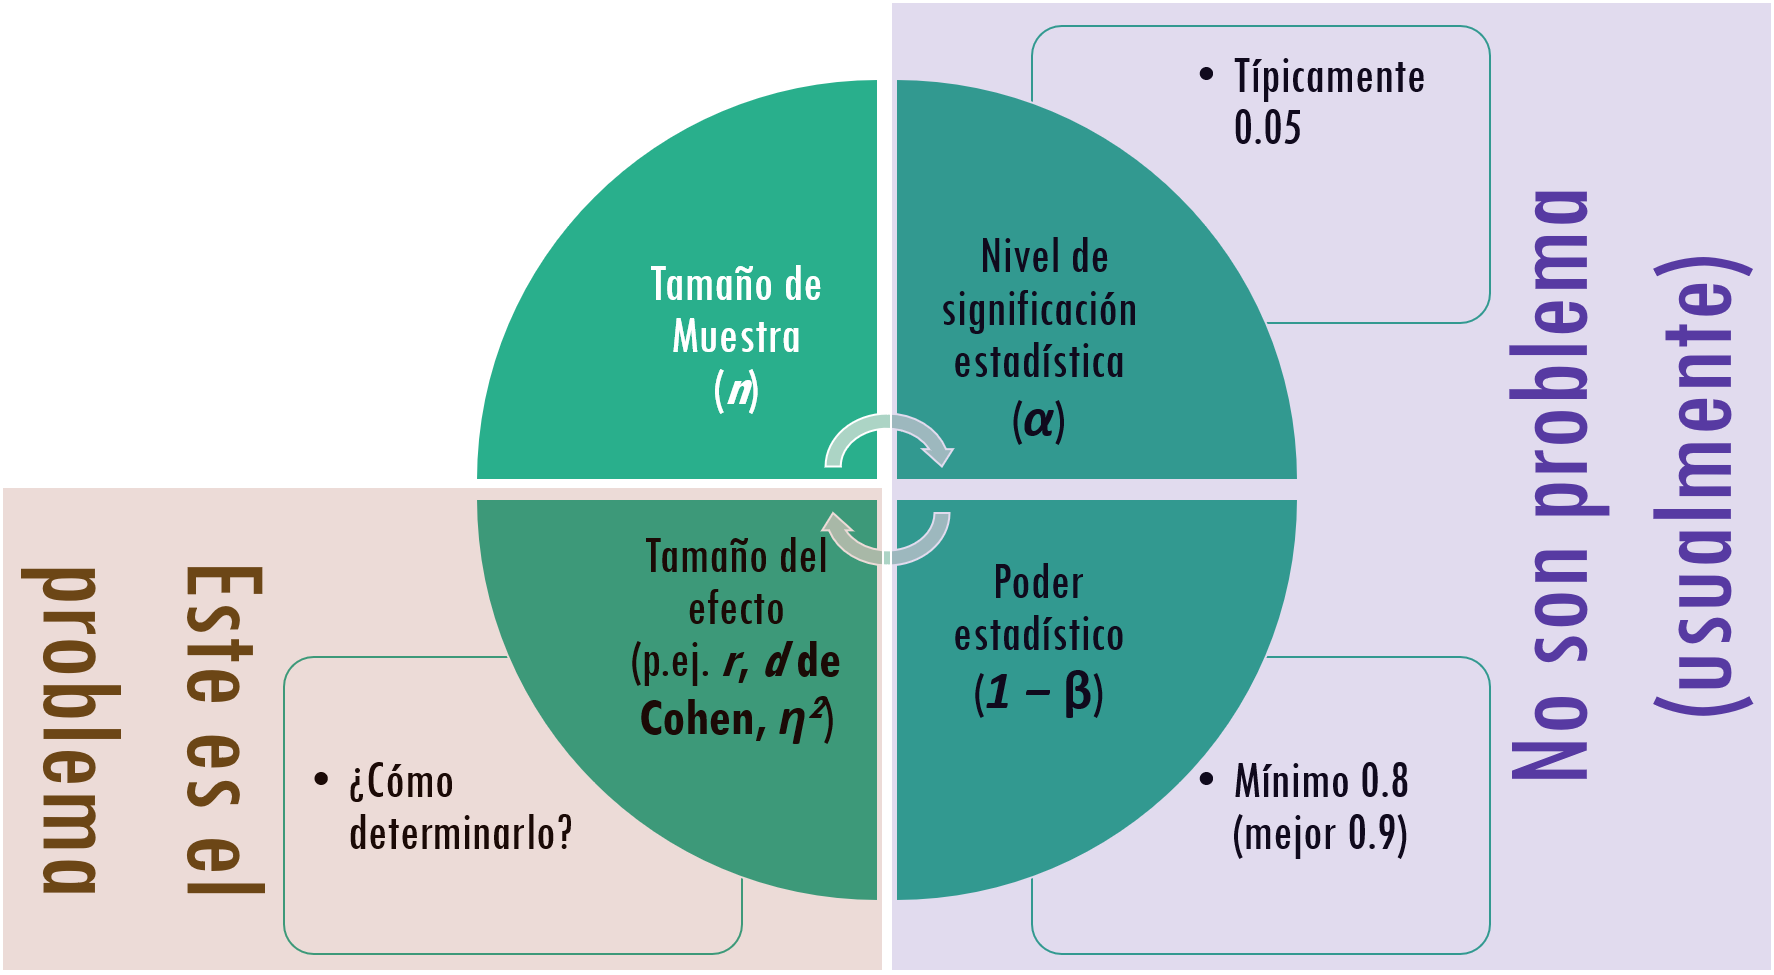
\includegraphics[width=450px]{4parametros} 

}

\caption{\textbf{Figura 1.} Parámetros necesarios para calcular el tamaño de muestra necesario, para obtener un poder estadístico deseado.}\label{fig:fig1}
\end{figure}

\hypertarget{probs}{%
\subsubsection{Por qué no es buena idea usar las definiciones de Cohen
(tamaños de efecto ``pequeños'', ``medios'' o
``grandes'')}\label{probs}}

Cohen (\protect\hyperlink{ref-cohenStatisticalPowerAnalysis1988}{1988},
\protect\hyperlink{ref-cohenPowerPrimer1992}{1992}) propuso unas
definiciones para las medidas de tamaños del efecto (``\emph{tamaños de
camiseta}'': efectos ``pequeños'', ``medios'' y ``grandes''). Consciente
de las limitaciones, él mismo advierte que su uso debe ser cuidadoso y
que su utilidad es relativa. Cohen planteó estas definiciones solo como
último recurso, cuando no hay evidencia previa que permita al
investigador estimar el tamaño de un efecto que va a estudiar. Sin
embargo, el uso indiscriminado y poco reflexivo de estas definiciones es
terriblemente frecuente.

El uso indiscriminado de las definiciones de las \emph{``camisetas''} es
problemático por dos razones fundamentales: las definiciones son
arbitrarias y son inconsistentes.

A pesar de que la mayoría de los tests estadísticos comunes
(pruebas-\emph{t}, correlaciones, regresiones lineales simples y
múltiples, ANOVAs y demás), hacen parte del mismo grupo de tests
(modelos lineales generales), existe una variedad de tamaños de efecto
estandarizados. Por ejemplo, típicamente se usa \(d\) de Cohen para
pruebas \emph{t}, \(r\) para correlaciones y regresiones simples, \(f\)
de Cohen o \(\eta^2\) para ANOVAs, y \(f^2\) para regresiones
múltiples\footnote{El \(f^2\) puede ser calculado de manera sencilla a
  partir del \(R^2\) de una regresión, con la ecuación
  \(f^2 = \frac{R^2}{1-R^2}\) (ver
  \protect\hyperlink{ref-selyaPracticalGuideCalculating2012}{Selya et
  al., 2012}).}. Esta variedad de tamaños de efecto hace que sea difícil
su comparación y su comprensión\footnote{Correll et al.
  (\protect\hyperlink{ref-correllAvoidCohenSmall2020}{2020}) han
  sugerido usar un único tamaño de efecto para todas estas pruebas, y
  sugieren que sea \(\eta^2\) (eta al cuadrado) dada su relativa
  facilidad para ser interpretado, su generalizabilidad, y que puede ser
  aplicado tanto a predictores continuos (problemáticos para medidas
  como \(d\) y \(f\)), como a predictores categóricos (problemáticos
  para \(r\)).}, y cada una tiene definiciones de ``pequeño'', ``medio''
y ``grande'' no congruentes (ver \textbf{Tabla 1}), que incluso llevan a
investigadores a calcular diferentes tamaños de muestra para el mismo
estudio, dependiendo de la prueba estadística que se va a
usar\footnote{Es común que unos datos puedan ser analizados de más de
  una manera; por ejemplo, puedo hacer una prueba-\emph{t} o una
  regresión, que me darían el mismo resultado para los mismos datos,
  pero las definiciones de ``pequeño'', ``medio'' y ``grande'' me
  sugerirían un tamaño de muestra diferente para obtener el mismo poder
  estadístico. De hecho, por ejemplo, si quiero obtener un efecto
  ``medio'' con una prueba-\emph{t} (\(d\) de Cohen = 0.5), el análisis
  de poder me sugeriría un \emph{n} = 128, muestras que una regresión
  (\(r\) = 0.30), me sugeriría un \emph{n} = 82. ¡Para analizar los
  mismos datos!}
(\protect\hyperlink{ref-correllAvoidCohenSmall2020}{Correll et al.,
2020}). En la \textbf{Tabla 1}, se ven las diferencias entre tamaños de
efecto comunes, de acuerdo con el porcentaje de varianza explicada.

\begin{table}[H]

\caption{\label{tab:tab1}\textbf{Tabla 1.} Diferencias en la varianza explicada por las definiciones de Cohen para diferentes tamaños de efecto.}
\centering
\resizebox{\linewidth}{!}{
\begin{threeparttable}
\begin{tabular}[t]{>{}cc>{}cc>{}cc>{}cc>{}c}
\toprule
\multicolumn{1}{c}{ } & \multicolumn{2}{c}{Prueba-$t$} & \multicolumn{2}{c}{ANOVA/ANCOVA} & \multicolumn{2}{c}{Correlación/Regresión Simple} & \multicolumn{2}{c}{Regresión múltiple} \\
\cmidrule(l{3pt}r{3pt}){2-3} \cmidrule(l{3pt}r{3pt}){4-5} \cmidrule(l{3pt}r{3pt}){6-7} \cmidrule(l{3pt}r{3pt}){8-9}
\makecell[c]{Definición \\de Cohen} & \makecell[c]{$d$ \\de Cohen} & \makecell[c]{Varianza \\explicada} & \makecell[c]{$f$ \\de Cohen} & \makecell[c]{Varianza \\explicada} & \makecell[c]{$r$ \\de Pearson} & \makecell[c]{Varianza \\explicada} & \makecell[c]{$f^2$ \\de Cohen} & \makecell[c]{Varianza \\explicada}\\
\midrule
\textbf{Pequeño} & 0.2 & \textbf{1\%} & 0.10 & \textbf{1\%} & 0.1 & \textbf{1\%} & 0.20 & \textbf{2\%}\\
\textbf{Medio} & 0.5 & \textbf{6\%} & 0.25 & \textbf{6\%} & 0.3 & \textbf{9\%} & 0.15 & \textbf{13\%}\\
\textbf{Grande} & 0.8 & \textbf{16\%} & 0.40 & \textbf{14\%} & 0.5 & \textbf{25\%} & 0.35 & \textbf{26\%}\\
\bottomrule
\end{tabular}
\begin{tablenotes}
\item \textit{Nota:} 
\item Las diferencias en la varianza explicada muestran que, aunque todas estas pruebas están relacionadas al ser todas modelos lineales generales, las definiciones propuestas por Cohen como tamaños de efecto "pequeños", "medios" o "grandes" difieren. Esto termina en que, para unos mismos datos, un análisis de poder termina por sugerir tamaños de muestra distintos, según el tamaño del efecto usado.
\end{tablenotes}
\end{threeparttable}}
\end{table}

Recientemente, Correll et al.
(\protect\hyperlink{ref-correllAvoidCohenSmall2020}{2020}) han hecho una
profunda e interesante revisión de los análisis de poder y cálculo de
tamaño de muestra, resaltando las limitaciones de las técnicas comunes,
así como sus alternativas.

\hypertarget{tuxe9cnicas-comunes-y-sus-limitaciones}{%
\subsubsection{Técnicas comunes y sus
limitaciones:}\label{tuxe9cnicas-comunes-y-sus-limitaciones}}

\begin{enumerate}
\def\labelenumi{\arabic{enumi}.}
\tightlist
\item
  \textbf{Definiciones de Cohen (tamaños de efecto ``pequeños'',
  ``medios'' o ``grandes'').} Fueron diseñados por Cohen
  (\protect\hyperlink{ref-cohenStatisticalPowerAnalysis1988}{1988},
  \protect\hyperlink{ref-cohenPowerPrimer1992}{1992}) solo como una guía
  cuando definitivamente no se tiene idea del tamaño del efecto que se
  va a estudiar. Sin embargo, son terriblemente problemáticos (ver
  \protect\hyperlink{ref-correllAvoidCohenSmall2020}{Correll et al.,
  2020}), y lastimosamente suelen usarse de manera casi automática.
  Además de la inconsistencia entre definiciones para diferentes medidas
  de tamaño del efecto (\textbf{Tabla 1}), su principal y más obvia
  limitación es que lo que se considera un efecto ``pequeño'' o
  ``grande'' cambia substancialmente entre disciplinas. Las definiciones
  propuestas por Cohen son percentiles (o cuartiles) de tamaños de
  efecto (25\% percentil, 50\% percentil o mediana, y 75\% percentil,
  como tamaños de efecto ``pequeños'', ``medios'' o ``grandes'',
  respectivamente). Si uno mira la literatura publicada, estos valores
  tienden a ser más o menos ciertos, pero dado que la literatura tiene
  sesgos, y que muchos se basan de por sí en estas definiciones, es
  difícil saber qué tan acertado es este método en un caso particular.
  En todo caso, estas definiciones no tienen por qué ser relevantes para
  un estudio que yo esté diseñando. Por esto, no se deben usar de manera
  indiscriminada, pues es muy posible que no sean válidos para el
  estudio que estoy diseñando. De hecho, recientemente, se ha
  argumentado que su uso no solo debe evitarse, sino que debe ser
  descartado completamente
  (\protect\hyperlink{ref-correllAvoidCohenSmall2020}{Correll et al.,
  2020}).
\item
  \textbf{Usar el tamaño del efecto de un único estudio previo.} Tiene
  un gran potencial de ser sesgado, dados los sesgos de publicación (los
  resultados nulos tienden a no ser publicados).
\item
  \textbf{Hacer un estudio piloto.} Esta técnica tiene sesgos implícitos
  y tiende a crear tamaños de efecto inflados, como ha sido demostrado
  (\protect\hyperlink{ref-albersWhenPowerAnalyses2018}{Albers \& Lakens,
  2018}). Sin embargo, si no hay estudios previos, podría ser una última
  opción para tener una indicación del poder estadístico esperado, pero
  asumiendo y reconociendo sus múltiples limitaciones.
\end{enumerate}

\hypertarget{alternativas}{%
\subsubsection{Alternativas}\label{alternativas}}

\begin{enumerate}
\def\labelenumi{\arabic{enumi}.}
\item
  \textbf{Ver la distribución de tamaños para un efecto particular:}
  \href{https://www.dsquintana.com/}{Daniel S. Quintana}, investigador
  en Psiquiatría Biológica de la Universidad de Oslo en Noruega propuso,
  cuando sea posible, ver la distribución de tamaños del efecto en un
  campo de estudio
  (\protect\hyperlink{ref-quintanaStatisticalConsiderationsReporting2017}{Quintana,
  2017}). En su artículo, Quintana analizó casi 300 estudios (y tamaños
  de efecto), para el campo de variabilidad de la frecuencia cardíaca, y
  calculó la distribución con base en percentiles (25\%, 50\% o mediana,
  y 75\%, a la manera de Cohen, pero aplicado directamente a su campo de
  estudio). Sin embargo, como él mismo menciona en
  \href{https://youtu.be/ZIjOG8LTTh8}{este video}, esta técnica, aunque
  tiende a ser menos sesgada que basarse en un único estudio previo, es
  todavía sujeta al sesgo que tengan los artículos en los que se basa,
  al igual que ocurre con meta-análisis. \newline \newline Entonces,
  aunque tiene limitaciones, esto es mejor que usar un único estudio
  publicado, usar un estudio piloto, o las definiciones de Cohen para
  estimar el tamaño del efecto que estoy estudiando. Sin embargo, puede
  no ser posible, cuando se trata de campos de estudio donde pocos
  estudios, o ninguno, han mirado el efecto que quiero estudiar, con
  diseños comparables. \newline \newline De nuevo, no hay una solución
  sencilla. Idealmente, el efecto que quiero usar para calcular el
  tamaño de muestra, debería ser el mismo (o muy cercano) al que de
  hecho encuentre al analizar mis datos.
\item
  \textbf{Determinar el ``menor tamaño de efecto de interés'':}. El
  ``menor tamaño de efecto de interés'' (en inglés, \emph{smallest
  effect size of interest} o \emph{SESOI}) es el tamaño mínimo de un
  efecto que se consideraría tiene importancia real. Esto se puede hacer
  tanto de manera objetiva, como subjetiva
  (\protect\hyperlink{ref-lakensEquivalenceTestingPsychological2018a}{Lakens,
  Scheel, et al., 2018}). En ese caso, se deberían rechazar efectos
  menores a ese mínimo justificado\footnote{Esto, sin embargo, no
    permite encontrar soporte para una hipótesis nula para lo cual se
    deben hacer tests de equivalencia (ver
    \protect\hyperlink{ref-lakensEquivalenceTestsPractical2017}{Lakens,
    2017}), algo que excede el enfoque de este documento.}.
  \newline \newline Esta es posiblemente la mejor opción, pues tiene en
  cuenta no solamente cuál es el tamaño de efecto esperado, sino también
  cuál es el mínimo tamaño de efecto que pueda resultar relevante para
  un efecto particular.
\end{enumerate}

Por otra parte, es importante saber que muchos tamaños de efecto pueden
ser comparables. Correll et al.
(\protect\hyperlink{ref-correllAvoidCohenSmall2020}{2020}) proponen usar
siempre el eta al cuadrado (\(\eta^2\)) como tamaño del efecto, y
presentan las ecuaciones, bastante sencillas\footnote{Son ecuaciones
  sencillas cuyos cálculos se pueden hacer en cualquier calculadora
  decente de celular o computador, o en \emph{Excel}, por ejemplo.},
para transformar medidas comunes de tamaños de efecto propuestos por
Cohen, desde o hacia \(\eta^2\) (\textbf{Tabla 2}).

\begin{table}[H]

\caption{\label{tab:tab2}\textbf{Tabla 2.} Conversión entre $\eta^2$ (eta al cuadrado) y medidas de tamaño de efecto de Cohen}
\centering
\begin{threeparttable}
\begin{tabular}[t]{>{}lcc}
\toprule
  & \makecell[c]{Tamaño de efecto de \\ Cohen a $\eta^2$} & \makecell[c]{$\eta^2$ a tamaño de \\ efecto de Cohen}\\
\midrule
\textbf{Prueba-$t$} & $\eta^2 = \frac{d^2}{d^2+4}$ & $d = \frac{2\sqrt{\eta^2}}{\sqrt{1-\eta^2}}$\\
\textbf{Correlación/Regresión Simple} & $\eta^2 = r^2$ & $r = \sqrt{\eta^2}$\\
\textbf{ANOVA/ANCOVA} & $\eta^2 = \frac{f^2}{1+f^2}$ & $f = \sqrt{\frac{\eta^2}{1-\eta^2}}$\\
\textbf{Regresión Múltiple} & $\eta^2 = \frac{f^2}{1+f^2}$ & $f^2 = \frac{\eta^2}{1-\eta^2}$\\
\bottomrule
\end{tabular}
\begin{tablenotes}
\item \textit{Nota:} 
\item Las ecuaciones de esta tabla reproducen las presentados en la Tabla 2 de Correll et al. (2020).
\end{tablenotes}
\end{threeparttable}
\end{table}

A continuación, presentaré algunas opciones de Software gratuito para
análisis de poder estadístico y tamaño de muestra.

\begin{center}\rule{0.5\linewidth}{0.5pt}\end{center}

\hypertarget{gpower}{%
\section{G*Power}\label{gpower}}

Probablemente la opción más común para hacer análisis de poder
estadístico y cálculos de tamaño de muestra es
\href{http://www.psychologie.hhu.de/arbeitsgruppen/allgemeine-psychologie-und-arbeitspsychologie/gpower.html}{G*Power}
(\protect\hyperlink{ref-faulPowerFlexibleStatistical2007}{Faul et al.,
2007}, \protect\hyperlink{ref-faulStatisticalPowerAnalyses2009}{2009}),
un software gratuito y relativamente sencillo. Sin embargo, la
terminología y documentación del programa son confusas y se prestan para
errores. De hecho, Correll et al.
(\protect\hyperlink{ref-correllAvoidCohenSmall2020}{2020}) afirman que
G*Power fomenta el uso de las definiciones de Cohen, pues permite al
investigador seleccionar una definición de tamaño con mínima
consideración de los temas relevantes, y sin tener en cuenta sus
numerosas y demostradas limitaciones (para una discusión de las
limitaciones de las definiciones de Cohen, ver sección
\protect\hyperlink{probs}{1.3.1 Por qué no es buena idea usar las
definiciones de Cohen}). Esto, sin embargo, no es problema siempre y
cuando el usuario del programa entienda los problemas de usar las
definiciones de Cohen, y evite o justifique muy bien su uso.

Adicionalmente, aunque menos importante, G*Power tiene limitaciones en
cuanto a los diseños para los cuales se pueden hacer análisis, en
especial cuando se trata de diseños factoriales, para los cuales sólo se
puede hacer análisis para efectos principales, o para una interacción,
pero solo para un efecto a la vez\footnote{En contraste, el paquete
  \texttt{Superpower} es capaz de hacer análisis de poder para diseños
  más complejos, y permite ver en un solo análisis los tamaños de
  muestra necesarios para efectos principales e interacciones. El uso de
  este paquete se describe en la sección
  \protect\hyperlink{Superpower}{7 Paquete \texttt{Superpower} para R}}.

Sin embargo, como ventaja, permite hacer análisis para una variedad de
pruebas estadísticas.

\begin{center}\rule{0.5\linewidth}{0.5pt}\end{center}

\hypertarget{jpower-muxf3dulo-de-jamovi}{%
\section{\texorpdfstring{\emph{jpower} (módulo de
\emph{jamovi})}{jpower (módulo de jamovi)}}\label{jpower-muxf3dulo-de-jamovi}}

Como alternativa, en \href{https://www.jamovi.org/}{\emph{jamovi}}
existe el paquete
\href{https://github.com/richarddmorey/jpower}{\emph{jpower}},
extremadamente claro y fácil de usar pero, hasta el momento, solo
permite análisis para diseños tipo prueba-\emph{t} (aunque está en
permanente desarrollo, y se está trabajando en incluir análisis de poder
para otros tipos de diseño). Adicionalmente, aunque hace unos reportes
muy claros y profesionales, que bien podrían ser adjuntados a cualquier
proyecto, por ahora solo los produce en inglés.

Si quieres ver mis videos acerca de \emph{jamovi}, y cómo instalarlo y
usarlo (con énfasis en la transición desde \emph{SPSS}), haz clic
\href{https://www.youtube.com/playlist?list=PLHk7UNt35ccXX4I61PiVMOf9VkijgaJN8}{acá}.

\hypertarget{tamauxf1o-del-efecto-en-jpower-para-jamovi-delta}{%
\subsection{\texorpdfstring{Tamaño del efecto en \emph{jpower} para
\emph{jamovi}:
\(\delta\)}{Tamaño del efecto en jpower para jamovi: \textbackslash delta}}\label{tamauxf1o-del-efecto-en-jpower-para-jamovi-delta}}

\emph{jpower} usa, como tamaño del efecto para pruebas-\emph{t}, el
\(\delta\) (delta) que es como se suele representar la diferencia
estandarizada entre dos medias a nivel de una población entera.

Es completamente equivalente a la \(d\) de Cohen (o \(g\) de hedges)
pero, a diferencia de la \(d\) de Cohen, hace referencia al tamaño de
efecto en la población entera, en vez de al efecto encontrado en una
muestra.

Entonces, dado que el \(\delta\) es un tamaño de efecto completamente
equivalente a la \(d\) de Cohen (o \(g\) de Hedges), pero que hace
referencia a una población, \emph{jamovi} nos está dando una pista: más
que simplemente poner la \(d\) encontrada en un estudio anterior, sería
ideal estimar el tamaño de efecto que esperamos (hipotetizamos) en la
población entera, o el tamaño de efecto mínimo que esperamos que exista
en la población entera, para estimar un tamaño de muestra que nos de un
poder estadístico suficiente para ese efecto (y, obviamente, un poder
mayor si el efecto fuese mayor).

Es importante tener en cuenta que, aunque la \(d\) de Cohen es el tamaño
del efecto más común para diferencias estandarizadas entre dos medias,
tiende a proporcionar estimaciones sesgadas cuando se tienen tamaños de
muestra pequeños\footnote{Esto se debe a que tanto la \(d\) de Cohen
  como la \(g\) de Hedges agrupan las varianzas (asumen que los grupos
  tienen la misma desviación estándar), pero la \(g\) de Hedges agrupa
  utilizando \(n - 1\) para cada muestra en lugar de \(n\), lo que
  proporciona una mejor estimación, especialmente cuanto menor es el
  tamaño de las muestras.} (\textbf{Figura 2}). Por este motivo, la
\(g\) de Hedges es siempre una alternativa valiosa que encontrarás en
muchos artículos (y que, sería mejor usar en todos los casos).

\begin{figure}
\centering
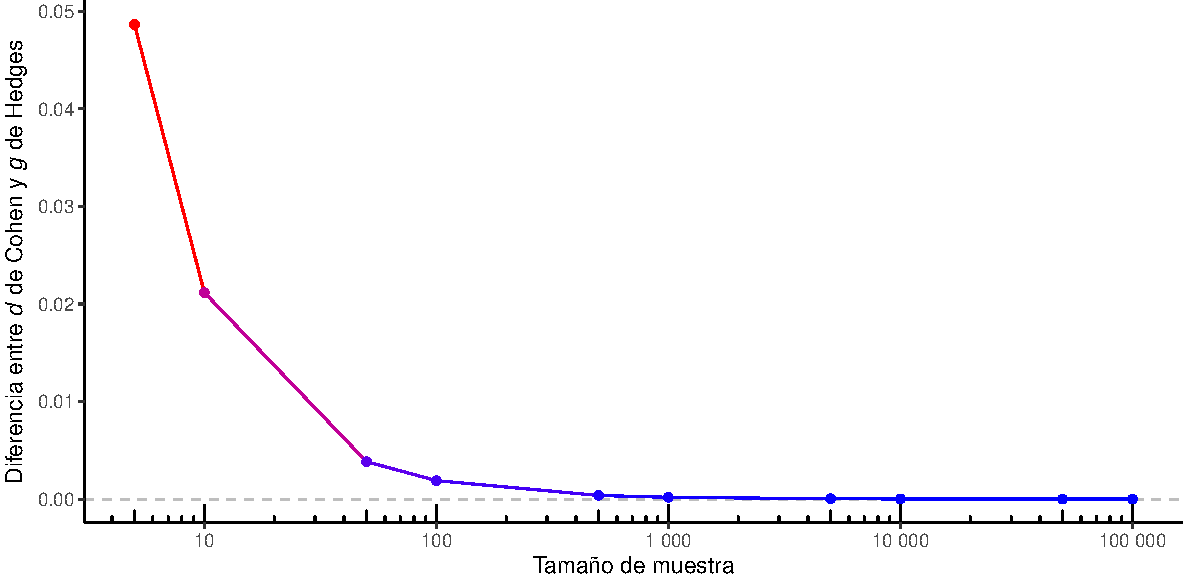
\includegraphics{PowerAnalysisScript_files/figure-latex/fig2-1.pdf}
\caption{\textbf{Figura 2.} Ejemplo de la diferencia entre el efecto
estimado como \emph{d} de Cohen versus el efecto estimado como \emph{g}
de Hedges (eje Y), según el tamaño de muestra (eje X). En muestras
péqueñas la \emph{d} de Cohen estima un efecto superior a la \emph{g} de
Hedges (en rojo), pero a medida que el tamaño de muestra aumenta (en
azul), la diferencia desaparece y tiende a 0 (línea gris). \emph{Nota:}
en este ejemplo, la diferencia entre las dos medias es 2 y la desviación
estándar es de 4.}
\end{figure}

\begin{center}\rule{0.5\linewidth}{0.5pt}\end{center}

\hypertarget{para-paquetes-de-r-instalaciuxf3n-de-r-y-rstudio}{%
\section{\texorpdfstring{Para paquetes de \emph{R}: instalación de
\emph{R} y
\emph{RStudio}}{Para paquetes de R: instalación de R y RStudio}}\label{para-paquetes-de-r-instalaciuxf3n-de-r-y-rstudio}}

\href{https://www.r-project.org/}{\emph{R}} puede parecer intimidante al
principio, pues requiere comandos (o \emph{``scripting''}), y a veces
incluso algo de programación. Sin embargo, es probablemente la mejor
herramienta que existe para hacer cualquier tipo de análisis de datos, y
con certeza supera por mucho a los \emph{software} comerciales (como
\emph{SPSS} y \emph{Stata}), que además suelen ser costosos.

Primero, \emph{R} es un software completamente \textbf{libre} y
\textbf{gratuito} y, al ser abierto, sus avances y funciones no están
limitados por lo que una compañía implemente (típicamente con fines
comerciales y sujeto a las leyes de oferta y demanda), sino que depende
directamente del trabajo colaborativo, y sin ánimo de lucro, de millones
de personas alrededor del mundo; por esto, avanza más rápido que
cualquier \emph{software} comercial, y siempre tiene opciones para poder
implementar las técnicas más novedosas\footnote{Prácticamente cada
  \emph{nerd} que desarrolla una nueva prueba o técnica de análisis de
  datos, hace, además de una publicación, un paquete para \emph{R}.}.
Segundo, al ser en últimas un lenguaje de programación, permite hacer
prácticamente cualquier cosa que se pueda hacer en un
computador\footnote{Solo como un ejemplo, este documento en PDF,
  \href{https://jdleongomez.info/es/}{mi sitio web}, y
  \href{https://jdleongomez.info/es/files/jdl_cv_es.pdf}{mi hoja de
  vida}, fueron todos creados en \emph{R}.}, explotando realmente sus
capacidades.

No puedo enfatizar de manera suficiente cuánto recomiendo, a cualquier
persona que trabaje con datos, aprender a usar \emph{R} (u otro lenguaje
comparable, como \href{https://www.python.org/}{\emph{Phyton}}), tanto
por la calidad y eficiencia de los análisis, como por las posibilidades
y ventajas laborales que esto da en el mundo de hoy.

Para usar los paquetes de \emph{R}, se necesita por supuesto tener el
programa instalado. Así mismo, recomiendo instalar y usar \emph{R} a
través de \href{https://rstudio.com/}{\emph{RStudio}}, pues facilita
enormemente la interacción con \emph{R}.

Para instalar \emph{R} y/o \emph{RStudio}, hay muchos tutoriales. Si
tienes que hacerlo, te recomiendo buscar videos en YouTube, donde hay
variedad de opciones (ninguna creada por mí hasta ahora) para todos los
sistemas operativos, incluyendo Windows (por ejemplo
\href{https://www.youtube.com/watch?v=D9Bp11iZssc}{este video}), Mac
(por ejemplo \href{https://www.youtube.com/watch?v=UCPr3W_wR5I}{este
video}), y Ubuntu (por ejemplo
\href{https://www.youtube.com/watch?v=PFlLatx5mlQ}{este video}).

En las siguientes secciones, el código de
\href{https://www.r-project.org/}{\emph{R}} está siempre resaltado sobre
un fondo oscuro. Para correr estos códigos, puedes sencillamente
copiarlos y pegarlos en un \emph{script}\footnote{\href{https://youtu.be/ejQ0BS2gVJI}{Este
  video}, hecho por
  \href{https://docentes.konradlorenz.edu.co/2019/06/juan-carlos-correa.html}{Juan
  Carlos Correa} (\protect\hyperlink{ref-correaScriptsVideo2020}{2020}),
  es un ejemplo de introducción al uso de \emph{scripts} de \emph{R}
  pero por supuesto hay muchos disponibles.}, o directamente en la
consola de \href{https://www.r-project.org/}{\emph{R}}.

\hypertarget{datos-usados-en-los-ejemplos-de-paquetes-de-r}{%
\section{\texorpdfstring{Datos usados en los ejemplos de paquetes de
\emph{R}}{Datos usados en los ejemplos de paquetes de R}}\label{datos-usados-en-los-ejemplos-de-paquetes-de-r}}

Todos los datos usados en los ejemplos de cómo usar las funciones
descritas en las siguientes secciones son generados de manera aleatoria,
y en ningún caso buscan representan estudios realizados, hechos, o
situaciones reales. En todos los casos, son datos creados y usados con
el único propósito de ilustrar de manera clara y didáctica el proceso de
realizar algunos análisis de poder, y calcular el tamaño de muestra
necesario para estudios hipotéticos.

\begin{center}\rule{0.5\linewidth}{0.5pt}\end{center}

\hypertarget{paquete-pwr-para-r-diseuxf1os-sencillos}{%
\section{\texorpdfstring{Paquete \emph{pwr} para \emph{R} (Diseños
sencillos)}{Paquete pwr para R (Diseños sencillos)}}\label{paquete-pwr-para-r-diseuxf1os-sencillos}}

\href{https://www.rdocumentation.org/packages/pwr/versions/1.3-0}{\texttt{pwr}}
(\protect\hyperlink{ref-champelyPwrBasicFunctions2020}{Champely et al.,
2020}) es un paquete flexible, claro, y muy confiable. Sin embargo, es
importante señalar que, al menos por ahora, solo permite hacer análisis
para diseños sencillos, incluyendo correlaciones y regresiones (simples
o múltiples), pruebas-\emph{t}, y ANOVAs de una vía (hasta el momento no
permite hacer análisis para diseños factoriales).

A continuación, mostraré algunos ejemplos de funciones para hacer
análisis de poder, y sus argumentos.

\hypertarget{instalaciuxf3n-y-carga-de-pwr}{%
\subsection{\texorpdfstring{Instalación y carga de
\texttt{pwr}}{Instalación y carga de pwr}}\label{instalaciuxf3n-y-carga-de-pwr}}

Para instalar y cargar \texttt{pwr}, se requiere correr las siguientes
funciones:

\begin{enumerate}
\def\labelenumi{\arabic{enumi}.}
\item
  Para instalar: \texttt{install.packages}, poniendo como argumento el
  nombre del paquete a instalar (en este caso, ``\texttt{pwr}'')
  \textbf{entre comillas}. Una vez el paquete ha sido instalado, no es
  necesario volver a usar esta función, excepto si el paquete se quiere
  reinstalar, o actualizar en un computador.
\item
  Para cargar: \texttt{library}, poniendo como argumento el nombre del
  paquete a cargar. Acá no es necesario poner el nombre entre comillas
  (pero no hay problema si se hace).
\end{enumerate}

En este caso, para instalar y cargar \texttt{pwr}, los comandos serían:

\begin{Shaded}
\begin{Highlighting}[]
\FunctionTok{install.packages}\NormalTok{(}\StringTok{"pwr"}\NormalTok{) }\CommentTok{\#para instalar el paquete (no es necesario si ya ha sido instalado).}
\FunctionTok{library}\NormalTok{(pwr) }\CommentTok{\#para cargar el paquete una vez instalado.}
\end{Highlighting}
\end{Shaded}

\hypertarget{niveles-de-referencia-de-los-tamauxf1os-del-efecto.-funciuxf3n-cohen.es}{%
\subsection{\texorpdfstring{Niveles de referencia de los tamaños del
efecto. Función
\texttt{cohen.ES}}{Niveles de referencia de los tamaños del efecto. Función cohen.ES}}\label{niveles-de-referencia-de-los-tamauxf1os-del-efecto.-funciuxf3n-cohen.es}}

El paquete \emph{pwr} tiene una función que podría resultar útil cuando
no hay información respecto al tamaño del efecto esperado, pero que debe
ser usada con cautela y buen criterio\footnote{Como discutí extensamente
  (ver sección \protect\hyperlink{probs}{1.3.1 Por qué no es buena idea
  usar las definiciones de Cohen}), Cohen
  (\protect\hyperlink{ref-cohenStatisticalPowerAnalysis1988}{1988},
  \protect\hyperlink{ref-cohenPowerPrimer1992}{1992}) propuso
  definiciones de referencia para los tamaños de efecto (efectos
  ``pequeños'', ``medios'', y ``grandes''), pero hay múltiples problemas
  con su uso indiscriminado.}. Se trata de la función \texttt{cohen.ES},
que permite rápidamente saber cuáles son las definiciones de referencia
para diferentes tamaños del efecto. Esta sencilla función solo tiene dos
argumentos: \emph{test} y \emph{size}.

\begin{enumerate}
\def\labelenumi{\arabic{enumi}.}
\item
  \texttt{test}: permite definir el tipo de tamaño del efecto que
  necesito. Las opciones incluyen ``t'', para pruebas-\emph{t}, ``r''
  para correlaciones, ``anov'' para ANOVAs de una vía (usando \emph{f}
  de Cohen como medida del tamaño del efecto), y ``f2'' para regresiones
  múltiples (en referencia al \(f^2\)).
\item
  \texttt{size}: permite definir el valor de referencia que quiero
  obtener. Las opciones son ``small'', ``medium'', y ``large'', para
  obtener el valor de referencia para el tamaño del efecto deseado
  pequeño, medio o grande, respectivamente.
\end{enumerate}

Por ejemplo, si quisiera saber cuál es el valor de referencia para una
correlación con un efecto pequeño, usaría:

\begin{Shaded}
\begin{Highlighting}[]
\FunctionTok{cohen.ES}\NormalTok{(}\AttributeTok{test =} \StringTok{"r"}\NormalTok{, }\AttributeTok{size =} \StringTok{"small"}\NormalTok{)}
\end{Highlighting}
\end{Shaded}

Esto produce:

\begin{verbatim}
## 
##      Conventional effect size from Cohen (1982) 
## 
##            test = r
##            size = small
##     effect.size = 0.1
\end{verbatim}

Donde, como se ve, me dice que el valor de referencia es \textbf{0.1}
(en el campo llamado ``\texttt{effect.size}'').

\hypertarget{anuxe1lisis-de-poder-para-correlaciones.-funciuxf3n-pwr.r.test}{%
\subsection{\texorpdfstring{Análisis de poder para correlaciones.
Función
\texttt{pwr.r.test}}{Análisis de poder para correlaciones. Función pwr.r.test}}\label{anuxe1lisis-de-poder-para-correlaciones.-funciuxf3n-pwr.r.test}}

Si, por ejemplo, quiero hacer un estudio, en el que espero determinar si
existe una correlación entre dos variables, para saber el tamaño de la
muestra (\emph{n}) adecuado, necesito entonces determinar:

\begin{enumerate}
\def\labelenumi{\arabic{enumi}.}
\tightlist
\item
  El tamaño del efecto (\emph{r}) esperado (es decir, qué tan fuerte es
  la asociación que espero entre las variables).
\item
  El alfa (\(\alpha\)) o nivel de significación estadística (típicamente
  0.05.).
\item
  El poder estadístico deseado (ver Sección
  \protect\hyperlink{power}{1.1 ¿Qué es Potencia o Poder Estadístico?}).
\end{enumerate}

Por ejemplo, si quiero tener 80\% de probabilidades de detectar como
significativa una correlación con un tamaño del efecto de \emph{r} =
0.3, con un \(\alpha\) = 0.05, puedo usar la siguiente función (en este
caso, \emph{``guardé''}\footnote{En realidad, como cualquier usuario
  habitual de \emph{R} sabe, lo que he hecho no es realmente
  \emph{``guardar''}, sino \textbf{\emph{asignar}} el resultado de la
  función a un objeto. Uso la palabra \emph{``guardar''} para
  simplificar la explicación para personas que no estén familiarizadas
  con \emph{R}, u otros lenguajes de programación, ya que los objetos
  suelen estar ocultos en la mayoría de los programas comerciales, y no
  requieren que el usuario los manipule directamente.} el resultado de
la función en un objeto que llamé \texttt{pcorr}).

\begin{Shaded}
\begin{Highlighting}[]
\NormalTok{pcorr }\OtherTok{\textless{}{-}} \FunctionTok{pwr.r.test}\NormalTok{(}\AttributeTok{r =} \FloatTok{0.3}\NormalTok{, }
           \AttributeTok{sig.level =} \FloatTok{0.05}\NormalTok{,}
           \AttributeTok{power =} \FloatTok{0.9}\NormalTok{) }\CommentTok{\#0.8 es típico, pero algunas disciplinas usan 0.9, o incluso 0.99}
\end{Highlighting}
\end{Shaded}

Para ver el resultado, solo necesito \emph{correr} en R el nombre de mi
objeto.

\begin{Shaded}
\begin{Highlighting}[]
\NormalTok{pcorr}
\end{Highlighting}
\end{Shaded}

Lo que produce:

\begin{verbatim}
## 
##      approximate correlation power calculation (arctangh transformation) 
## 
##               n = 111.8068
##               r = 0.3
##       sig.level = 0.05
##           power = 0.9
##     alternative = two.sided
\end{verbatim}

Como se ve, en el campo llamado ``\texttt{n}'', me dice que la muestra
necesaria para obtener el poder deseado de 90\% para detectar como
significativa una correlación con un \emph{r} de 0.3, es de 111.8068.
Por supuesto, yo no puedo tener un número no entero de observaciones o
participantes, por lo que el valor \emph{n} (tamaño de muestra), debe
aproximarse al siguiente número entero superior (en este caso, 112).

Finalmente, puedo ver la asociación entre el tamaño de la muestra y el
poder estadístico gráficamente con la función \texttt{plot}\footnote{Las
  figuras que produce la función \texttt{plot} para análisis hechos en
  el paquete \texttt{pwr}, son objetos de clase \texttt{ggplot}, por lo
  que alguien familiarizado con el paquete
  \href{https://ggplot2.tidyverse.org/}{\texttt{ggplot2}} puede
  modificar la figura para que, por ejemplo, los ejes, título y
  anotaciones estén en español, o para cambiar el tema y colores.},
introduciendo como argumento mi objeto (en este caso \texttt{pcorr})
puedo ver una figura de este análisis (\textbf{Figura 3}).

\begin{Shaded}
\begin{Highlighting}[]
\FunctionTok{plot}\NormalTok{(pcorr)}
\end{Highlighting}
\end{Shaded}

\begin{figure}
\centering
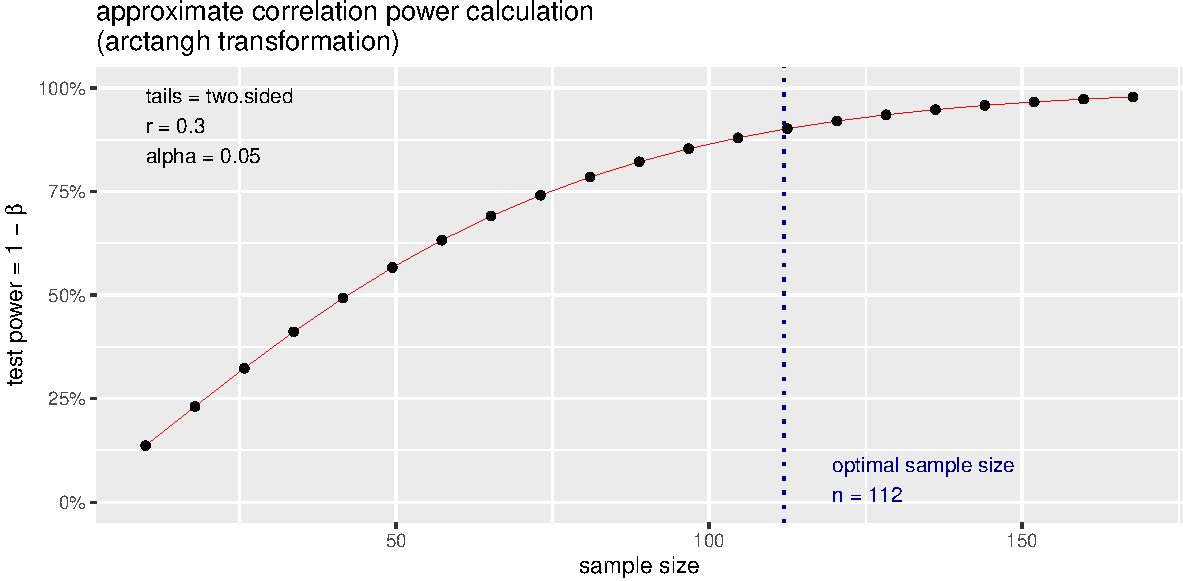
\includegraphics{PowerAnalysisScript_files/figure-latex/fig3-1.pdf}
\caption{\textbf{Figura 3.} Asociación entre el tamaño de la muestra y
el poder estadístico para una correlación de 0.3, con un \(\alpha\) de
0.05, producida con la función \texttt{plot} del paquete \texttt{pwr}.
Como se puede ver, sugiere un \emph{n} de 112 (línea azul), para
alcanzar un poder de 0.9 (90\%).}
\end{figure}

\hypertarget{si-hay-hipuxf3tesis-claras-pre-especificadas-a-priori-se-pueden-hacer-anuxe1lisis-de-una-cola}{%
\subsubsection{\texorpdfstring{Si hay hipótesis claras,
pre-especificadas (\emph{a priori}), se pueden hacer análisis de una
cola}{Si hay hipótesis claras, pre-especificadas (a priori), se pueden hacer análisis de una cola}}\label{si-hay-hipuxf3tesis-claras-pre-especificadas-a-priori-se-pueden-hacer-anuxe1lisis-de-una-cola}}

Cuando tengo una hipótesis precisa, como que la correlación que estudio
será positiva, puedo hacer análisis de una cola, lo que reduce
substancialmente el tamaño de muestra requerido. Sin embargo, esto solo
se debe hacer cuando tengo una hipótesis clara, con sólido fundamento
teórico, o empírico (por ejemplo, en el caso de una replicación).

Para hacerlo, el argumento \texttt{alternative} debe ser definido:

\begin{enumerate}
\def\labelenumi{\arabic{enumi}.}
\tightlist
\item
  \textbf{Para correlaciones positivas:}
  \texttt{alternative\ =\ "greater"}.
\item
  \textbf{Para correlaciones negativas:} \texttt{alternative\ =\ "less"}
  (en cuyo caso el argumento \texttt{r} \textbf{debe} ser negativo; por
  ejemplo -0.3).
\end{enumerate}

Por ejemplo, en este caso, al especificar que espero que el tamaño del
efecto sea positivo, y \textbf{al menos} de \emph{r} = 0.3, el \emph{n}
se reduce de 112 a 92 observaciones o participantes.

\begin{Shaded}
\begin{Highlighting}[]
\NormalTok{pcorrgreater }\OtherTok{\textless{}{-}} \FunctionTok{pwr.r.test}\NormalTok{(}\AttributeTok{r =} \FloatTok{0.3}\NormalTok{,}
                     \AttributeTok{sig.level =} \FloatTok{0.05}\NormalTok{,}
                     \AttributeTok{power =} \FloatTok{0.9}\NormalTok{,}
                     \AttributeTok{alternative =} \StringTok{"greater"}\NormalTok{) }\CommentTok{\#Depeniendo de si es positivo o negativo}
\NormalTok{pcorrgreater}
\end{Highlighting}
\end{Shaded}

\begin{verbatim}
## 
##      approximate correlation power calculation (arctangh transformation) 
## 
##               n = 91.41024
##               r = 0.3
##       sig.level = 0.05
##           power = 0.9
##     alternative = greater
\end{verbatim}

\textcolor{red}{\faBookmark} \textbf{Es importante tener en cuenta que
este análisis de poder de una cola únicamente tendrá sentido si mi
correlación es, de hecho, positiva.}

Al igual que antes, con la función \texttt{plot}, puedo ver una figura
de este análisis (\textbf{Figura 4}).

\begin{Shaded}
\begin{Highlighting}[]
\FunctionTok{plot}\NormalTok{(pcorrgreater)}
\end{Highlighting}
\end{Shaded}

\begin{figure}
\centering
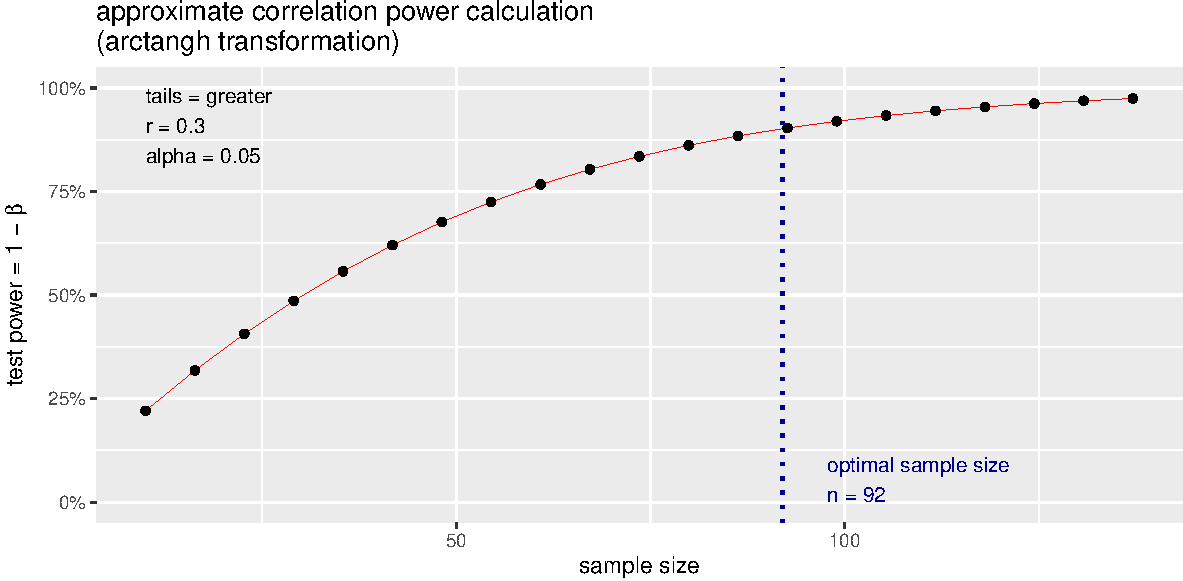
\includegraphics{PowerAnalysisScript_files/figure-latex/fig4-1.pdf}
\caption{\textbf{Figura 4.} Asociación entre el tamaño de la muestra y
el poder estadístico para una correlación \textbf{positiva} (de una
cola), de \textbf{al menos} 0.3, con un \(\alpha\) de 0.05, producida
con la función \texttt{plot} del paquete \texttt{pwr}. Como se puede
ver, sugiere un \emph{n} de 67 (línea azul), para alcanzar un poder de
0.9 (90\%).}
\end{figure}

\hypertarget{anuxe1lisis-de-poder-para-pruebas-t.-funciuxf3n-pwr.t.test}{%
\subsection{\texorpdfstring{Análisis de poder para pruebas-\emph{t}.
Función
\texttt{pwr.t.test}}{Análisis de poder para pruebas-t. Función pwr.t.test}}\label{anuxe1lisis-de-poder-para-pruebas-t.-funciuxf3n-pwr.t.test}}

Existen tres tipos de pruebas-\emph{t}: (1) pruebas-\emph{t} de muestras
independientes (o no relacionadas), que se usan por ejemplo cuando
comparo dos grupos de personas; (2) pruebas-\emph{t} de medidas
repetidas, relacionadas o pareadas, que se usan cuando comparo, por
ejemplo, al mismo grupo de personas en dos momentos (e.g.~antes y
después de un tratamiento), o en dos condiciones (e.g.~tomando una
medicina vs tomando un placebo); y (3) pruebas-\emph{t} de una muestra,
que se usan cuando comparo una serie de datos (por ejemplo la estatura
de un grupo particular de personas) con un valor ya conocido (e.g.~la
media de estatura establecida para país), para saber si los miembros de
mi grupo tienden a ser más bajos, más altos, o de altura similar a la
población general.

La función \texttt{pwr.t.test} asume por defecto que se trata de un
análisis de medidas independientes (\texttt{type\ =\ "two.sample"}), a
menos que se defina qué tipo de prueba-\emph{t} responde a mi diseño,
usando el argumento \texttt{type}:

\begin{enumerate}
\def\labelenumi{\arabic{enumi}.}
\tightlist
\item
  \textbf{Para pruebas-\emph{t} de muestras independientes:}
  \texttt{type\ =\ "two.sample"}.
\item
  \textbf{Para pruebas-\emph{t} de medidas repetidas:}
  \texttt{type\ =\ "paired"}.
\item
  \textbf{Para pruebas-\emph{t} de una muestra:}
  \texttt{type\ =\ "one.sample"}.
\end{enumerate}

\hypertarget{TInd}{%
\subsubsection{Muestras independientes}\label{TInd}}

En este caso, \emph{``guardé''} el resultado de la función en un objeto
que llamé \texttt{ptInd}.

\begin{Shaded}
\begin{Highlighting}[]
\NormalTok{ptInd }\OtherTok{\textless{}{-}} \FunctionTok{pwr.t.test}\NormalTok{(}\AttributeTok{d =} \FloatTok{0.4}\NormalTok{,}
                    \AttributeTok{sig.level =} \FloatTok{0.05}\NormalTok{,}
                    \AttributeTok{power =} \FloatTok{0.9}\NormalTok{,}
                    \AttributeTok{type =} \StringTok{"two.sample"}\NormalTok{)}
\NormalTok{ptInd }\CommentTok{\#los resultados son MUY claros en cuanto a que el n es para cada grupo.}
\end{Highlighting}
\end{Shaded}

Lo que produce:

\begin{verbatim}
## 
##      Two-sample t test power calculation 
## 
##               n = 132.3105
##               d = 0.4
##       sig.level = 0.05
##           power = 0.9
##     alternative = two.sided
## 
## NOTE: n is number in *each* group
\end{verbatim}

Al igual que con las correlaciones, con la función \texttt{plot}, puedo
ver una figura de este análisis (\textbf{Figura 5}).

\begin{Shaded}
\begin{Highlighting}[]
\FunctionTok{plot}\NormalTok{(ptInd)}
\end{Highlighting}
\end{Shaded}

\begin{figure}
\centering
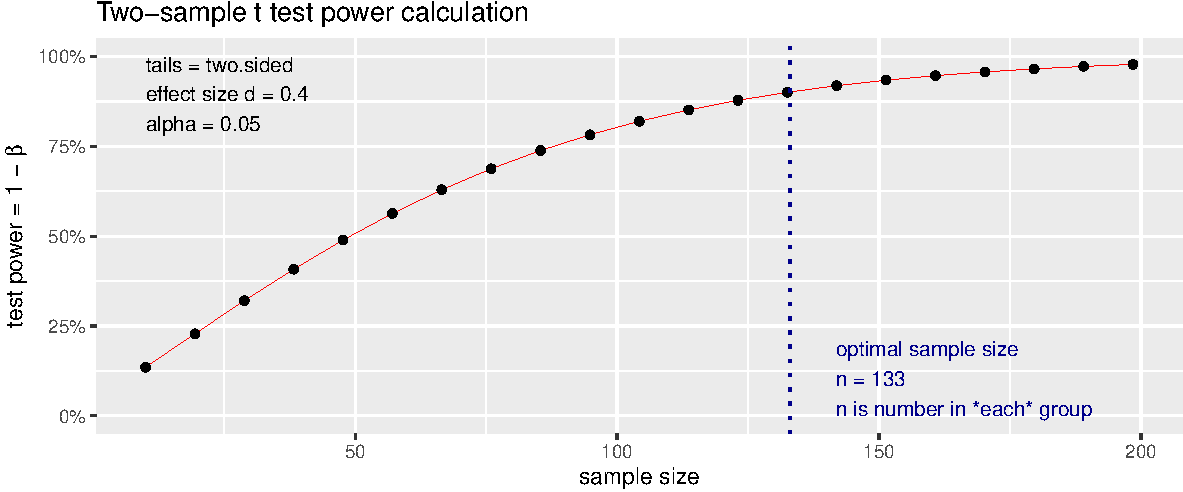
\includegraphics{PowerAnalysisScript_files/figure-latex/fig5-1.pdf}
\caption{\textbf{Figura 5.} Asociación entre el tamaño de la muestra y
el poder estadístico para una prueba-\emph{t} de 0.4, con un \(\alpha\)
de 0.05, producida con la función \texttt{plot} del paquete
\texttt{pwr}. Como se puede ver, sugiere un \emph{n} de 133 por grupo
(línea azul), para alcanzar un poder de 0.9 (90\%).}
\end{figure}

\hypertarget{una-muestra}{%
\subsubsection{Una muestra}\label{una-muestra}}

Para este ejemplo, \emph{``guardé''} el resultado de la función en un
objeto que llamé \texttt{ptUna}.

\begin{Shaded}
\begin{Highlighting}[]
\NormalTok{ptUna }\OtherTok{\textless{}{-}} \FunctionTok{pwr.t.test}\NormalTok{(}\AttributeTok{d =} \FloatTok{0.4}\NormalTok{, }\AttributeTok{sig.level =} \FloatTok{0.05}\NormalTok{,}
                    \AttributeTok{power =} \FloatTok{0.9}\NormalTok{,}
                    \AttributeTok{type =} \StringTok{"one.sample"}\NormalTok{)}
\NormalTok{ptUna}
\end{Highlighting}
\end{Shaded}

\begin{verbatim}
## 
##      One-sample t test power calculation 
## 
##               n = 67.62138
##               d = 0.4
##       sig.level = 0.05
##           power = 0.9
##     alternative = two.sided
\end{verbatim}

\hypertarget{TRep}{%
\subsubsection{Medidas repetidas o pareadas}\label{TRep}}

Es importante tener en cuenta que, de ser posible, suele ser mejor hacer
diseños de medidas repetidas, con respecto a medidas independientes,
pues en general esto representa un mejor uso de recursos: como son
análisis más poderosos estadísticamente, tienen un \emph{n} más pequeño
comparados con análisis equivalentes de medidas independientes.

Sin embargo, por supuesto no todas las preguntas pueden ser respondidas
con un análisis de medidas repetidas. Si por ejemplo quiero mirar
diferencias entre perros y gatos en la cantidad de atención prestada a
los humanos, no puedo tener a mis participantes una vez como perros, y
otra como gatos. En este ejemplo, no existe la opción de hacer medidas
repetidas, como tampoco existiría si quisiera comparar la capacidad
pulmonar (o cualquier otra variable) de personas nacidas en Uruguay y
personas nacidas en Panamá, pues por supuesto las personas solo nacen
una vez, y en un solo país.

En este caso, por ejemplo, mientras un análisis de medidas
independientes como el presentado antes (sección
\protect\hyperlink{TInd}{5.4.1 Muestras independientes}) requería un
\emph{n} de 133 personas por grupo (es decir, 266 en total), el mismo
análisis pero con un diseño de medidas repetidas requiere un \emph{n} de
68 personas (con dos observaciones por persona).

\begin{Shaded}
\begin{Highlighting}[]
\NormalTok{ptRep }\OtherTok{\textless{}{-}} \FunctionTok{pwr.t.test}\NormalTok{(}\AttributeTok{d =} \FloatTok{0.4}\NormalTok{,}
                    \AttributeTok{sig.level =} \FloatTok{0.05}\NormalTok{,}
                    \AttributeTok{power =} \FloatTok{0.9}\NormalTok{,}
                    \AttributeTok{type =} \StringTok{"paired"}\NormalTok{)}
\NormalTok{ptRep }\CommentTok{\#los resultados son MUY claros en cuanto a que el n es para pares de observaciones.}
\end{Highlighting}
\end{Shaded}

\begin{verbatim}
## 
##      Paired t test power calculation 
## 
##               n = 67.62138
##               d = 0.4
##       sig.level = 0.05
##           power = 0.9
##     alternative = two.sided
## 
## NOTE: n is number of *pairs*
\end{verbatim}

\hypertarget{anuxe1lisis-de-una-cola}{%
\subsubsection{Análisis de una cola}\label{anuxe1lisis-de-una-cola}}

De nuevo, cuando tenemos una hipótesis precisa, como que la diferencia
entre grupos estudiados será en una dirección particular (e.g.~Grupo 2
\textgreater{} Grupo 1), se pueden hacer análisis de una cola, tanto
para pruebas-\emph{t} de medidas independientes, relacionadas, o de una
muestra, lo que reduce substancialmente el tamaño de muestra requerido.

Para hacerlo, el argumento \texttt{alternative} debe ser definido:

\begin{enumerate}
\def\labelenumi{\arabic{enumi}.}
\tightlist
\item
  \textbf{Para diferencias positivas (donde Gr 2 \textgreater{} Gr 1):}
  \texttt{alternative\ =\ "greater"}.
\item
  \textbf{Para correlaciones negativas (donde Gr 2 \textless{} Gr 1):}
  \texttt{alternative\ =\ "less"} (en cuyo caso el argumento \texttt{d}
  también \textbf{debe} ser negativo; por ejemplo -0.3).
\end{enumerate}

Por ejemplo, en este caso, al especificar que espero que el tamaño del
efecto de medidas repetidas (sección \protect\hyperlink{TRep}{5.4.3
Muestras repetidas o pareadas}) sea positivo, y con un \emph{d} de Cohen
de \textbf{al menos} 0.4, el \emph{n} se reduce de 68 a 55 pares de
observaciones (es decir, 55 participantes, cada uno medido 2 veces).

\begin{Shaded}
\begin{Highlighting}[]
\NormalTok{ptRepGreat }\OtherTok{\textless{}{-}} \FunctionTok{pwr.t.test}\NormalTok{(}\AttributeTok{d =} \FloatTok{0.4}\NormalTok{,}
                    \AttributeTok{sig.level =} \FloatTok{0.05}\NormalTok{,}
                    \AttributeTok{power =} \FloatTok{0.9}\NormalTok{,}
                    \AttributeTok{type =} \StringTok{"paired"}\NormalTok{,}
                    \AttributeTok{alternative =} \StringTok{"greater"}\NormalTok{)}
\NormalTok{ptRepGreat}
\end{Highlighting}
\end{Shaded}

\begin{verbatim}
## 
##      Paired t test power calculation 
## 
##               n = 54.90553
##               d = 0.4
##       sig.level = 0.05
##           power = 0.9
##     alternative = greater
## 
## NOTE: n is number of *pairs*
\end{verbatim}

\textcolor{red}{\faBookmark} \textbf{Es importante tener en cuenta que
este análisis de una cola análisis únicamente tendrá sentido si mi
correlación es, de hecho, positiva.}

Al igual que antes, con la función \texttt{plot}, puedo ver una figura
de este análisis (\textbf{Figura 6}).

\begin{Shaded}
\begin{Highlighting}[]
\FunctionTok{plot}\NormalTok{(ptRepGreat)}
\end{Highlighting}
\end{Shaded}

\begin{figure}
\centering
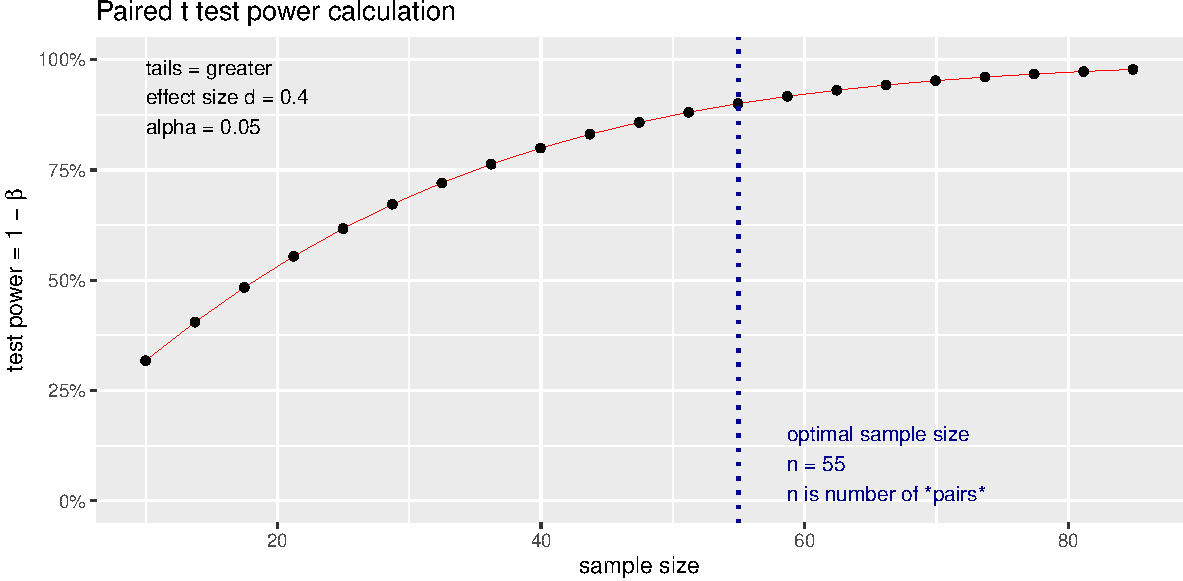
\includegraphics{PowerAnalysisScript_files/figure-latex/fig6-1.pdf}
\caption{\textbf{Figura 6.} Asociación entre el tamaño de la muestra y
el poder estadístico para una prueba-\emph{t} de \textbf{al menos} 0.4
(una cola), con un \(\alpha\) de 0.05, producida con la función
\texttt{plot} del paquete \texttt{pwr}. Como se puede ver, sugiere un
\emph{n} de 55 (línea azul), para alcanzar un poder de 0.9 (90\%).}
\end{figure}

\hypertarget{anuxe1lisis-de-poder-para-anovas-de-una-vuxeda.-funciuxf3n-pwr.anova.test}{%
\subsection{\texorpdfstring{Análisis de poder para ANOVAs de una vía.
Función
\texttt{pwr.anova.test}}{Análisis de poder para ANOVAs de una vía. Función pwr.anova.test}}\label{anuxe1lisis-de-poder-para-anovas-de-una-vuxeda.-funciuxf3n-pwr.anova.test}}

Por lo menos hasta ahora\footnote{La versión actual de \texttt{pwr} es
  la 1.3-0.}, \texttt{pwr} solo permite hacer análisis de poder para
ANOVAs de una vía, balanceados (mismo número de participantes u
observaciones por grupo), y de medidas independientes (es decir,
comparando un número \emph{k} de grupos)\footnote{Para diseños más
  complejos, incluyendo diseños factoriales de medidas independientes,
  repetidas, o mixtas (tanto factores de medidas independientes como
  repetidas), la mejor opción actualmente es el paquete
  \texttt{Superpower}, descrito en la siguiente sección.}.

Los argumentos de esta función son similares a los de las funciones
\texttt{pwr.r.test} y \texttt{pwr.t.test}:

\begin{enumerate}
\def\labelenumi{\arabic{enumi}.}
\tightlist
\item
  \texttt{k}: número de grupos a comparar en mi ANOVA de una vía.
\item
  \texttt{f}: tamaño del efecto (\emph{f} de Cohen) esperado (es decir,
  qué tan fuerte es la asociación que espero entre la variable
  independiente, que divide mis grupos, y la variable dependiente).
\item
  \texttt{sig.level}: alfa (\(\alpha\)) o nivel de significación
  estadística (típicamente 0.05.).
\item
  \texttt{power}: poder estadístico deseado (ver sección
  \protect\hyperlink{power}{1.1 ¿Qué es Potencia o Poder Estadístico?}).
\end{enumerate}

Los argumentos \texttt{sig.level} y \texttt{power} son iguales, y se
usan de manera idéntica en esta función que en las funciones
\texttt{pwr.r.test} y \texttt{pwr.t.test}.

El tamaño del efecto también se usa de manera similar, pero con la
diferencia de que para la función \texttt{pwr.anova.test} se define un
tamaño \emph{f}, mientras que para \texttt{pwr.r.test} y
\texttt{pwr.t.test} se usaban tamaños del efecto \emph{r} y \emph{t},
respectivamente.

Sin embargo, la función \texttt{pwr.anova.test} tiene algunos cambios:

\begin{enumerate}
\def\labelenumi{\arabic{enumi}.}
\tightlist
\item
  \texttt{k} es un argumento nuevo, que se usa para definir el número de
  grupos a comparar. Este argumento no se usaba en la función
  \texttt{pwr.t.test} para pruebas-\emph{t} de este paquete.
\item
  \texttt{alternative} y \texttt{type}, argumentos usados en la función
  \texttt{pwr.t.test} para pruebas-\emph{t} de este paquete, no se usan
  para esta función.
\end{enumerate}

Entonces, teniendo esto en cuenta, si por ejemplo quiero alcanzar un
poder \(1 - \beta\) de 0.9 (90\%), con un \(\alpha\) de 0.05, para
detectar un \emph{f} de 0.25, al comparar 4 grupos, es necesario un
\emph{n} de 58 participantes en cada grupo (o 232 participantes en
total, dado que el diseño propuesto tendría 4 grupos).

\begin{Shaded}
\begin{Highlighting}[]
\NormalTok{panova }\OtherTok{\textless{}{-}} \FunctionTok{pwr.anova.test}\NormalTok{(}\AttributeTok{k =} \DecValTok{4}\NormalTok{,}
                         \AttributeTok{f =} \FloatTok{0.25}\NormalTok{,}
                         \AttributeTok{sig.level =} \FloatTok{0.05}\NormalTok{,}
                         \AttributeTok{power =} \FloatTok{0.9}\NormalTok{)}
\NormalTok{panova}
\end{Highlighting}
\end{Shaded}

Lo que produce:

\begin{verbatim}
## 
##      Balanced one-way analysis of variance power calculation 
## 
##               k = 4
##               n = 57.67309
##               f = 0.25
##       sig.level = 0.05
##           power = 0.9
## 
## NOTE: n is number in each group
\end{verbatim}

Al igual que con las demás funciones para calcular el poder estadístico
del paquete \texttt{pwr}, con la función \texttt{plot}, puedo ver una
figura de este análisis.

\begin{Shaded}
\begin{Highlighting}[]
\FunctionTok{plot}\NormalTok{(panova)}
\end{Highlighting}
\end{Shaded}

\begin{figure}
\centering
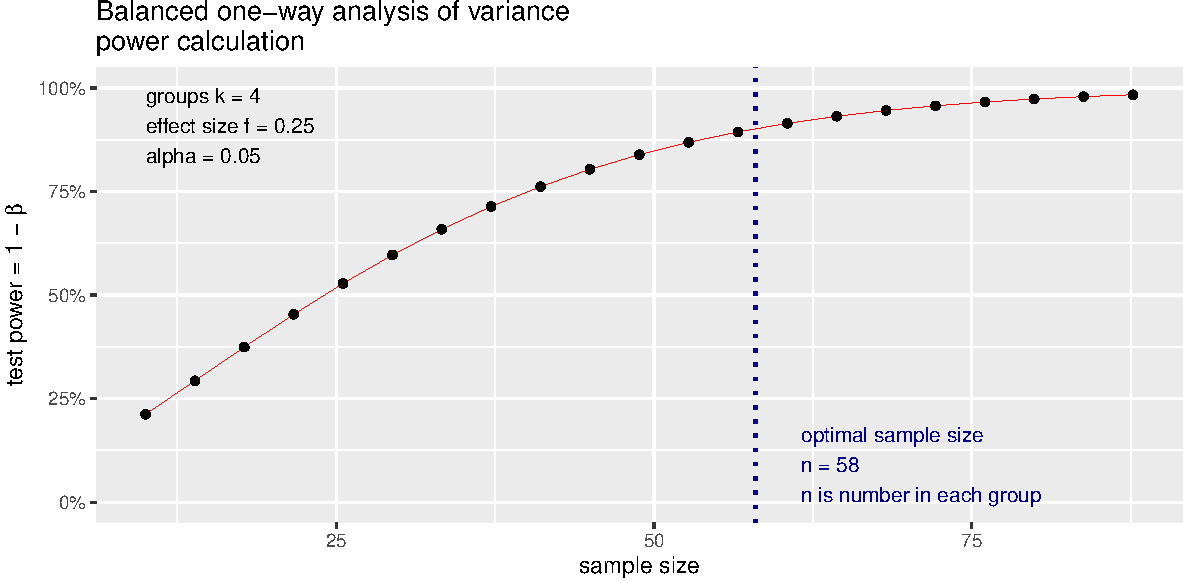
\includegraphics{PowerAnalysisScript_files/figure-latex/fig7-1.pdf}
\caption{\textbf{Figura 7.} Asociación entre el tamaño de la muestra y
el poder estadístico para un ANOVA de 0.4, con un \(\alpha\) de 0.05,
producida con la función \texttt{plot} del paquete \texttt{pwr}. Como se
puede ver, sugiere un \emph{n} de 58 participantes por grupo (línea
azul), para alcanzar un poder de 0.9 (90\%).}
\end{figure}

\begin{center}\rule{0.5\linewidth}{0.5pt}\end{center}

\hypertarget{Superpower}{%
\section{\texorpdfstring{Paquete \emph{Superpower} para \emph{R}
(diseños factoriales
complejos)}{Paquete Superpower para R (diseños factoriales complejos)}}\label{Superpower}}

El paquete
\href{https://cran.r-project.org/web/packages/Superpower/vignettes/intro_to_superpower.html}{\texttt{Superpower}}
(\protect\hyperlink{ref-caldwellSuperpowerSimulationBasedPower2020}{Caldwell
et al., 2020};
\protect\hyperlink{ref-caldwellPowerAnalysisSuperpower2020}{Caldwell \&
Lakens, 2020};
\protect\hyperlink{ref-lakensIntroductionSuperpower2020}{Lakens \&
Caldwell, 2020}), está específicamente diseñado para permitir hacer
análisis de poder para diseños de una vía o factoriales (con más de un
factor o variable independiente nominal), incluyendo diseños complejos,
de manera empírica. En esta guía, me centraré en los diseños
factoriales.

\hypertarget{diseuxf1os-factoriales}{%
\subsection{Diseños factoriales}\label{diseuxf1os-factoriales}}

En los diseños factoriales, normalmente hay más de un efecto de interés.
Por ejemplo, si quiero saber el efecto del género (hombre, mujer) y el
máximo nivel educativo (pregrado, postgrado), en el salario de los
médicos, podría hacer un diseño 2 \(\times\) 2. Esto quiere decir que
tengo dos factores (variables independientes nominales): el género y el
nivel educativo, cada uno con dos niveles (1. hombre y 2. mujer, para el
caso del género; y 1. pregrado y 2. postgrado, para el caso del nivel
educativo).

En este caso, yo obtendría 3 valores \emph{p}:

\begin{enumerate}
\def\labelenumi{\arabic{enumi}.}
\tightlist
\item
  Efecto principal del género, que me diría si hay diferencias en el
  salario entre hombres y mujeres.
\item
  Efecto principal del nivel educativo, que me dice si hay diferencias
  entre el salario de médicos con pregrado y médicos con postgrado como
  máximo nivel educativo alcanzado.
\item
  Interacción entre género y nivel educativo, que me dice si el salario
  depende simultáneamente del género y el nivel educativo. Por ejemplo,
  si entre las mujeres ganan más dinero las personas con postgrado, pero
  entre los hombres ganan más las personas con pregrado\footnote{Obviamente
    este ejemplo muy seguramente no representa la realidad. Es solamente
    un ejemplo hipotético.}.
\end{enumerate}

Por supuesto, yo podría tener diseños más complejos, como un 2
\(\times\) 4, donde tengo, de nuevo, 2 factores, pero uno que tiene 2
niveles, y otro que tiene 4. O un diseño 2 \(\times\) 2 \(\times\) 3,
donde hay 3 factores, con 2, 2, y 3 niveles, respectivamente.

Es importante tener en cuenta que, al aumentar el número de factores,
independientemente del número de niveles que tengan esos factores, el
número de resultados (y valores \emph{p} asociados) aumenta. Por
ejemplo, mientras en el caso de un diseño con dos factores hay 3
resultados, en un diseño con tres factores (voy a llamarlos \textbf{A},
\textbf{B} y \textbf{C}), hay 7:

\begin{enumerate}
\def\labelenumi{\arabic{enumi}.}
\tightlist
\item
  Efecto principal del primer factor (\textbf{A}).
\item
  Efecto principal del segundo factor (\textbf{B}).
\item
  Efecto principal del tercer factor (\textbf{C}).
\item
  Interacción entre el primer y segundo factor (\textbf{A} \(\times\)
  \textbf{B}).
\item
  Interacción entre el primer y tercer factor (\textbf{A} \(\times\)
  \textbf{C}).
\item
  Interacción entre el segundo y tercer factor (\textbf{B} \(\times\)
  \textbf{C})..
\item
  Interacción entre los tres factores (\textbf{A} \(\times\) \textbf{B}
  \(\times\) \textbf{C}).
\end{enumerate}

Dada la complejidad de estos cálculos, y la multiplicidad de efectos
(principales e interacciones) y resultados asociados, y dado que para
detectar cada uno de esos efectos hay un poder estadístico distinto, la
mayoría de los programas para análisis de poder solamente permiten
analizar un efecto a la vez. Por ejemplo, G*Power, aunque permite hacer
análisis de poder para diseños complejos, solo calcula un efecto a la
vez.

En contraste, el paquete \texttt{Superpower} permite hacer análisis, no
solo para diseños más complejos, sino calculando simultáneamente el
poder para cada efecto, y para posibles comparaciones \emph{post-hoc}.

Este proceso es sumamente complejo, y no se puede solucionar de manera
matemática \emph{sencilla}\footnote{No existe una única ecuación que
  permita hacer este cálculo.}, por lo que \texttt{Superpower} usa una
estrategia interesante: simula una base de datos para el diseño
propuesto (dadas una serie de características de cada variable y su
relación con las demás\footnote{En particular, se necesita saber la
  media y desviación estándar de cada grupo y/o condición y, cuando hay
  factores de medidas repetidas, una matriz de correlaciones entre cada
  combinación de niveles.}), y empíricamente estima el poder, a partir
de hacer muchas iteraciones (repeticiones aleatorias) de esta
simulación.

Dadas estas complejidades, en ocasiones no es posible tener la
información suficiente para hacer las simulaciones, pues se requiere de
estudios previos (o pilotos) muy completos, con diseños idénticos, y
que, o bien hayan reportado toda esta información, o hayan abierto
libremente sus bases de datos para poder hacer estos
cálculos\footnote{Esta es una de las razones por las cuales es muy
  importante que en cada artículo haya una sección de descriptivos muy
  buena y completa, e idealmente que los datos estén disponibles para
  poder re-analizarlos, o hacer este tipo de análisis descriptivos
  necesarios para hacer un análisis de poder}.

Por esto, la forma de usar \texttt{Superpower} y sus funciones, es muy
distinta a la de \texttt{pwr}. En las siguientes secciones mostraré
ejemplos de análisis de poder para diseños factoriales de medidas
independientes, repetidas y mixtas, pero por simplicidad siempre usaré
diseños 2 \(\times\) 2. Para diseños más complejos la lógica es, en todo
caso, la misma.

\hypertarget{instalaciuxf3n-y-carga-de-superpower}{%
\subsection{\texorpdfstring{Instalación y carga de
\texttt{Superpower}}{Instalación y carga de Superpower}}\label{instalaciuxf3n-y-carga-de-superpower}}

Para instalar y cargar \texttt{Superpower}, se requiere correr las
siguientes funciones:

\begin{Shaded}
\begin{Highlighting}[]
\FunctionTok{install.packages}\NormalTok{(}\StringTok{"Superpower"}\NormalTok{) }\CommentTok{\#no es necesario si ya ha sido instalado.}
\FunctionTok{library}\NormalTok{(Superpower) }\CommentTok{\#para cargar el paquete una vez instalado.}
\end{Highlighting}
\end{Shaded}

\hypertarget{multcomp}{%
\subsection{\texorpdfstring{Acerca de comparaciones
\emph{post-hoc}}{Acerca de comparaciones post-hoc}}\label{multcomp}}

Comúnmente, al hacer un ANOVA, bien sea de una vía o factorial, se deben
hacer además comparaciones \emph{post-hoc} {[}o, alternativamente,
\emph{contrastes planeados}; e.g. Chatham
(\protect\hyperlink{ref-chathamPlannedContrastsOverview1999}{1999}){]}
para determinar entre qué grupos o condiciones están las diferencias.
Por ejemplo, al hacer un ANOVA de una vía comparando cuatro grupos, si
el resultado del ANOVA es significativo, es probable que quiera
determinar si hay diferencias entre los grupos 1 y 2, 1 y 4, o 3 y 4,
por ejemplo.

Es importante tener en cuenta que el número de comparaciones
\emph{post-hoc} posibles para un ANOVA aumenta rápidamente cuando tengo
más factores, o los factores tienes más niveles (independientemente de
que estos factores sean de medidas repetidas o independientes).

De hecho, el número de posibles comparaciones (que he denominado
\(n_{comp}\)) es el producto de los niveles de todos los factores al
cuadrado menos el producto de esos mismos niveles, dividido por dos.
Entonces:

Para un diseño 2 \(\times\) 2 (o un diseño con un solo factor con 4
niveles) hay 6 comparaciones posibles:

\[n_{comp} = \frac{(2 \times 2)^2-(2 \times 2)}{2} = \frac{16-4}{2} = 6\]

Para un diseño 3 \(\times\) 2 (o un diseño con un solo factor con 6
niveles) hay 15 comparaciones posibles:

\[n_{comp} = \frac{(3 \times 2)^2-(3 \times 2)}{2} = \frac{36-6}{2} = 15\]

Para un diseño 2 \(\times\) 2 \(\times\) 2, hay 28 comparaciones
posibles:

\[n_{comp} = \frac{(2 \times 2 \times 2)^2-(2 \times 2 \times 2)}{2} = \frac{64-8}{2} = 28\]

Para un diseño 3 \(\times\) 2 \(\times\) 2, hay 66 comparaciones
posibles:

\[n_{comp} = \frac{(3 \times 2 \times 2)^2-(3 \times 2 \times 2)}{2} = \frac{144-12}{2} = 66\]

Y para un diseño 2 \(\times\) 2 \(\times\) 4 (que tendría el mismo
número de comparaciones que un diseño 2 \(\times\) 2 \(\times\) 2
\(\times\) 2), hay 120 comparaciones posibles:

\[n_{comp} = \frac{(2 \times 2 \times 4)^2-(2 \times 2 \times 4)}{2} = \frac{256-16}{2} = 120\]

Esto es muestra de cómo la complejidad de los diseños, especialmente
factoriales, aumenta exponencialmente al tener más factores, o más
niveles por factor.

\hypertarget{holm}{%
\subsubsection{\texorpdfstring{Cómo controlar la tasa de errores al
hacer pruebas \emph{post-hoc}. Correcciones de \emph{Bonferroni} y
\emph{Holm-Bonferroni}}{Cómo controlar la tasa de errores al hacer pruebas post-hoc. Correcciones de Bonferroni y Holm-Bonferroni}}\label{holm}}

Hacer pruebas \emph{post-hoc} o cualquier tipo de comparaciones
múltiples sobre la misma base de datos, aunque importante, infla la tasa
de errores Tipo I (falsos positivos), por lo que generalmente se hacen
correcciones al \(\alpha\) (nivel de significación), para contrarrestar
esta mayor posibilidad de encontrar diferencias que, en realidad, no
existan.

En otras palabras, dado que si tengo un \(\alpha\) = 0.05, estoy
aceptando una probabilidad de que el 5\% (o 1 de cada 20) resultados sea
falso, si hago dos análisis, la probabilidad de un falso positivo de
dobla (10\%), si hago 3 se triplica (15\%), etcétera. Si hago 20
análisis, estoy probabilísticamente asegurando que obtendré un falso
resultado positivo. Y si hago un ANOVA \(2 \times 2 \times 4\), con sus
120 comparaciones \emph{post-hoc}, probabilísticamente obtendría seis
falsos positivos.

Para contrarrestar este problema, existen varias opciones, de las cuales
probablemente la más conocida es la \emph{corrección de Bonferroni}
(\protect\hyperlink{ref-bonferroniTeoriaStatisticaClassi1936}{Bonferroni,
1936}), que consiste en reducir el \(\alpha\) (típicamente de 0.05),
dividiéndolo por el número de comparaciones múltiples (o pruebas
\emph{post-hoc}) que se hagan.

Entonces, si por ejemplo hago dos comparaciones \emph{post-hoc},
\(\alpha = \frac{0.05}{2} = 0.025\), y si hago seis,
\(\alpha = \frac{0.05}{6} = 0.0083\). Esto, por supuesto, hace que sea
más difícil encontrar resultados significativos (en efecto, reduciendo
el poder estadístico, que es la probabilidad de detectar como
significativo un efecto que sí existe). Por esto, aunque la
\emph{corrección de Bonferroni} controla muy bien la tasa de errores
Tipo I (falsos positivos), infla la tasa de errores Tipo II (falsos
negativos), dejando como única alternativa incrementar el tamaño de la
muestra (y por consiguiente, el poder estadístico).

Sin embargo, existen alternativas más modernas y versátiles (para una
revisión y comparación, ver
\protect\hyperlink{ref-blakesleyComparisonsMethodsMultiple2009}{Blakesley
et al., 2009}). De estas, una relativamente sencilla y popular,
disponible en muchos paquetes estadísticos, es la \emph{corrección de
Holm-Bonferroni}
(\protect\hyperlink{ref-holmSimpleSequentiallyRejective1979a}{Holm,
1979}). Esta alternativa, que personalmente me gusta mucho, es una
suerte de \emph{corrección de Bonferroni} pero aplicada secuencialmente.

Es decir, si por ejemplo hago seis comparaciones \emph{post-hoc},
\(\alpha = \frac{0.05}{6} = 0.0083\) se aplicará para el efecto con el
valor \emph{p} más pequeño, \(\alpha = \frac{0.05}{5} = 0.01\) al
segundo más pequeño, \(\alpha = \frac{0.05}{4} = 0.0125\) al tercero más
pequeño, \(\alpha = \frac{0.05}{3} = 0.0167\) al cuarto más pequeño,
\(\alpha = \frac{0.05}{2} = 0.025\) al quinto más pequeño, y
\(\alpha = \frac{0.05}{1} = 0.05\) al sexto más pequeño (que sería el
valor \emph{p} más grande).

Al hacer esta corrección secuencial, a \emph{corrección de
Holm-Bonferroni} tiene la ventaja de limitar la inflación de la tasa de
errores Tipo II (falsos negativos), en comparación a la \emph{corrección
de Bonferroni} (ver e.g.
\protect\hyperlink{ref-streinerBestOftforgottenPractices2015}{Streiner,
2015}), sin dejar de controlar la tasa de errores Tipo I (falsos
positivos) .

Como explicaré en las siguientes secciones, el paquete
\texttt{Superpower} permite calcular en un solo análisis el poder
estadístico, tanto de los efectos principales e interacciones, como
también para las comparaciones \emph{post-hoc}, implementando al tiempo
correcciones de \emph{Bonferroni}, \emph{Holm-Bonferroni}, u otras
opciones disponibles.

\hypertarget{ind}{%
\subsection{ANOVA factorial de medidas independientes}\label{ind}}

En todos los casos, los análisis de poder requieren \textbf{al menos}
dos funciones:

\begin{enumerate}
\def\labelenumi{\arabic{enumi}.}
\item
  \texttt{ANOVA\_design} que permite especificar las características del
  diseño para el cual haré el análisis de poder.
\item
  Una función para obtener el análisis de poder con base en el diseño.
  Para esto, hay varias opciones, incluyendo\footnote{El paquete
    \texttt{Superpower} tiene otras funciones muy útiles para análisis
    de poder estadístico, que por simplicidad no cubriré en este
    documento. Para conocerlas, recomiendo ver la
    \href{https://www.rdocumentation.org/packages/Superpower/versions/0.0.3}{documentación
    del paquete}, o la
    \href{https://cran.r-project.org/web/packages/Superpower/vignettes/intro_to_superpower.html}{introducción}
    hecha por los autores al mismo
    (\protect\hyperlink{ref-lakensIntroductionSuperpower2020}{Lakens \&
    Caldwell, 2020}).}:

  \begin{itemize}
  \tightlist
  \item
    \texttt{ANOVA\_power} que usa simulaciones para determinar el poder
    estadístico obtenido.
  \item
    \texttt{plot\_power} que muestra gráficamente el poder obtenido
    según el tamaño de la muestra (similar a la función \texttt{plot} de
    \texttt{pwr}), pero para todos los efectos principales e
    interacciones.
  \end{itemize}
\end{enumerate}

\hypertarget{ejemplo-anova-factorial-de-medidas-independientes-2-times-2}{%
\subsubsection{\texorpdfstring{Ejemplo ANOVA factorial de medidas
independientes (2 \(\times\)
2)}{Ejemplo ANOVA factorial de medidas independientes (2 \textbackslash times 2)}}\label{ejemplo-anova-factorial-de-medidas-independientes-2-times-2}}

Entonces, si por ejemplo quiero estudiar los resultados de un examen de
matemáticas entre estudiantes becados y no becados, de universidades
públicas y privadas, tengo un diseño 2 (Beca: 1. Sí, 2. No) \(\times\) 2
(Universidad: 1. Pública, 2. Privada).

Para hacer este análisis, debo primero definir el diseño y las
características del mismo con la función \texttt{ANOVA\_design}.

Para esto, requiero los siguientes argumentos:

\begin{enumerate}
\def\labelenumi{\arabic{enumi}.}
\item
  \texttt{design}: este argumento esencial, define el tipo de diseño. En
  este caso, dado que tengo un diseño 2 \(\times\) 2, donde ambos
  factores son de medidas independientes, debo ponerlo como
  \texttt{"2b*2b"}, donde los números representan el número de niveles
  en cada factor, la letra \textbf{b} que ese factor en de medidas
  independientes (o \emph{entre sujetos}, por lo cual usa la letra
  \textbf{b}, del inglés \emph{between-subjects}.)
\item
  \texttt{n}: el número de participantes que espero tener por por
  condición (o, dicho de otro modo, por combinación de niveles entre mis
  factores; e.g.~(1) estudiantes becados de universidades privadas; (2)
  estudiantes becados de universidades públicas, etcétera). Aunque, a
  diferencia de otros paquetes y programas, \texttt{Superpower} no
  calcula el \emph{n} por mí, me permite cambiar el \emph{n} hasta
  lograr el poder deseado.
\item
  \texttt{mu}: las medias para cada interacción entre los niveles de mis
  factores. En este caso, (1) la media de estudiantes becados de
  universidades públicas, (2) estudiantes becados de universidades
  privadas, (3) estudiantes no becados de universidades públicas, y (4)
  estudiantes becados de universidades privadas. Estos valores, como se
  verá en el código, deben estar \emph{concatenados} usando la función
  \texttt{c}.
\item
  \texttt{sd}: la desviación estándar para la población (por lo cual es
  un solo valor. En este caso, la desviación estándar de las
  calificaciones del examen).
\item
  \texttt{labelnames} (Opcional): las etiquetas (nombres) de los
  factores y sus niveles. Al igual que con las medias, estas
  etiquetas\footnote{Estos nombres o etiquetas no deben contener
    espacios.} deben estar \emph{concatenadas} usando la función
  \texttt{c}. Para definirlos, se deben poner en el siguiente orden:

  \begin{itemize}
  \tightlist
  \item
    Etiqueta del primer factor (en este caso ``Beca'')
  \item
    Etiquetas de los niveles de ese factor (en este caso ``Sí'' y
    ``No'')
  \item
    Etiqueta del segundo factor (en este caso ``Universidad'')
  \item
    Etiquetas de los niveles de ese factor (en este caso ``Pública'' y
    ``Privada'')
  \end{itemize}
\item
  \texttt{plot} (Opcional): este es un argumento lógico que únicamente
  acepta como opciones \texttt{TRUE} y \texttt{FALSE"}. Si incluyo
  \texttt{plot\ =\ TRUE} esta función creará además una figura
  (\emph{plot}) mostrando las medias y sus intervalos de confianza (si
  no incluyo este argumento, por defecto la función asumirá la opción
  \texttt{FALSE} y no producirá esta figura.)
\end{enumerate}

Entonces, el código para este diseño hipotético sería el siguiente, con
80 participantes en cada combinación de \emph{Beca} y \emph{Universidad}
(320 en total), si los puntajes promedio (\texttt{mu}) del examen fuesen
57 (becados de universidad pública), 62 (becados de universidad
privada), 53 (no becados de universidad pública), y 44 (no becados de
universidad privada), con una desviación estándar (\texttt{sd}) de
15.4\footnote{Por supuesto, estos datos son hipotéticos y no representan
  ningún estudio real, ni diferencias entre estudiantes con y sin beca,
  ni entre universidades públicas y privadas. Solo son usados como un
  ejemplo.}.

\begin{Shaded}
\begin{Highlighting}[]
\NormalTok{disenoB }\OtherTok{\textless{}{-}} \FunctionTok{ANOVA\_design}\NormalTok{(}\AttributeTok{design =} \StringTok{"2b*2b"}\NormalTok{,}
                       \AttributeTok{n =} \DecValTok{80}\NormalTok{, }\AttributeTok{sd =} \FloatTok{15.4}\NormalTok{,}
                       \AttributeTok{mu =} \FunctionTok{c}\NormalTok{(}\DecValTok{57}\NormalTok{, }\DecValTok{62}\NormalTok{, }\DecValTok{53}\NormalTok{, }\DecValTok{44}\NormalTok{),}
                       \AttributeTok{labelnames =} \FunctionTok{c}\NormalTok{(}\StringTok{"Beca"}\NormalTok{, }\StringTok{"Sí"}\NormalTok{, }\StringTok{"No"}\NormalTok{, }\StringTok{"Universidad"}\NormalTok{, }\StringTok{"Púbica"}\NormalTok{, }\StringTok{"Privada"}\NormalTok{),}
                       \AttributeTok{plot =} \ConstantTok{TRUE}\NormalTok{)}
\end{Highlighting}
\end{Shaded}

\begin{figure}
\centering
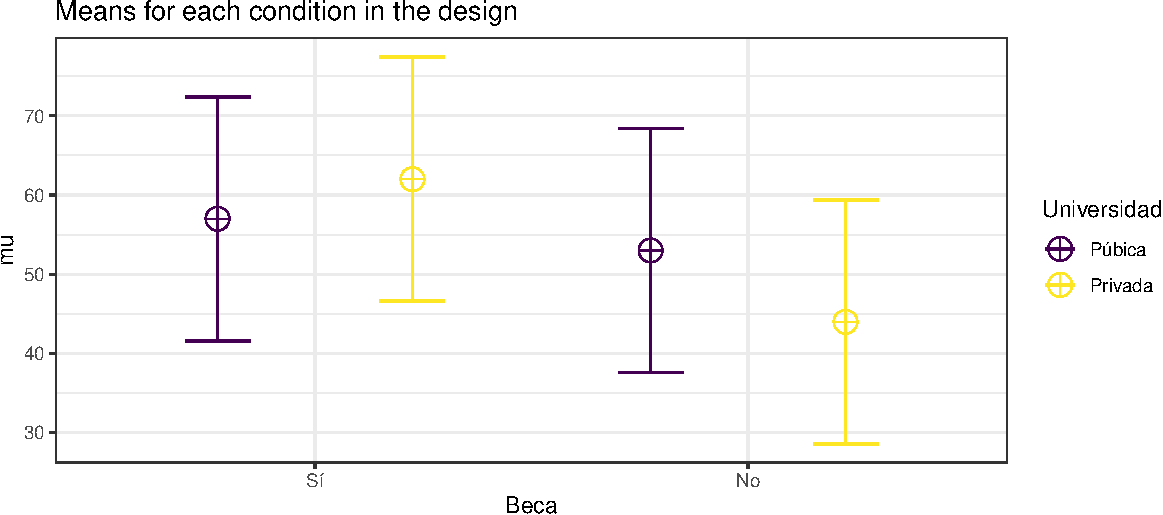
\includegraphics{PowerAnalysisScript_files/figure-latex/fig8-1.pdf}
\caption{\textbf{Figura 8.} Ejemplo de la distribución de medias y sus
intervalos de confianza para el diseño definido con la función
\texttt{ANOVA\_design}, al incluir el argumento \texttt{plot\ =\ TRUE}.
Esto es muy útil para estar seguro de que las medias fueron
\emph{concatenadas} en el orden correcto.}
\end{figure}

Definido el diseño y las características de los datos
(\emph{``guardando''} este diseño en un objeto que llamé
\texttt{disenoB}), puedo ver el poder que obtendría con esos 80
participantes por cada combinación de \emph{Beca} y \emph{Universidad},
con la función \texttt{ANOVA\_power}.

Esta función, además de requerir como argumento el diseño que acabo de
definir (en este caso \texttt{disenoB}), requiere que defina:

\begin{enumerate}
\def\labelenumi{\arabic{enumi}.}
\tightlist
\item
  \texttt{alpha\_level}: \(\alpha\) (nivel de significación) deseado.
  Típicamente 0.05.
\item
  \texttt{p.adjust}: si se debe hacer un ajuste para comparaciones
  \emph{post-hoc} (por ejemplo correcciones de \emph{Bonferroni} con la
  opción \texttt{"bonferroni"}, \emph{Holm-Bonferroni} con la opción
  \texttt{"holm"}, o sin corrección, usando la opción \texttt{"none"};
  para ver todas las opciones, recomiendo ver la documentación de la
  función
  \href{https://www.rdocumentation.org/packages/stats/versions/3.6.2/topics/p.adjust}{\texttt{p.adjust}}).
  En este caso definí que quiero hacer una corrección de
  ``\texttt{holm}'', que se refiere a la corrección de
  \emph{Holm-Bonferroni}
  (\protect\hyperlink{ref-holmSimpleSequentiallyRejective1979a}{Holm,
  1979}).
\item
  \texttt{nsim}: número de simulaciones hechas para determinar el poder;
  acá es importante tener en cuenta que un número mayor de simulaciones
  me dará resultados más robustos y confiables, pero requerirá más
  tiempo. Los autores del paquete recomiendan usar mínimo 100
  simulaciones
  (\protect\hyperlink{ref-lakensIntroductionSuperpower2020}{Lakens \&
  Caldwell, 2020}).
\item
  \texttt{seed} (opcional): Adicionalmente, para el siguiente ejemplo
  usé el argumento \texttt{seed} para que las simulaciones den siempre
  el mismo resultado\footnote{Dado que las bases de datos se simulan con
    base en las características definidas con la función
    \texttt{ANOVA\_design}, pero \textbf{de manera aleatoria}, cada vez
    que corra la función obtendré un resultado ligeramente distinto,
    especialmente si el número de simulaciones (\texttt{nsim}) es
    pequeño. Al darle una semilla (\texttt{seed}), que puede ser
    cualquier número, los datos simulados siempre serán los mismos,
    garantizando que la respuesta sea la misma.}.
\end{enumerate}

El código entonces quedaría de la siguiente manera:

\begin{Shaded}
\begin{Highlighting}[]
\FunctionTok{ANOVA\_power}\NormalTok{(disenoB, }
            \AttributeTok{alpha\_level =} \FloatTok{0.05}\NormalTok{,}
            \AttributeTok{p\_adjust =} \StringTok{"holm"}\NormalTok{, }
            \AttributeTok{seed =} \DecValTok{2019}\NormalTok{, }
            \AttributeTok{nsims =} \DecValTok{1000}\NormalTok{)}
\end{Highlighting}
\end{Shaded}

Lo que produce:

\begin{verbatim}
## Power and Effect sizes for ANOVA tests
##                        power effect_size
## anova_Beca             100.0    0.117825
## anova_Universidad       24.0    0.007927
## anova_Beca:Universidad  98.3    0.052368
## 
## Power and Effect sizes for pairwise comparisons (t-tests)
##                                                           power effect_size
## p_Beca_Sí_Universidad_Púbica_Beca_Sí_Universidad_Privada   50.3      0.3180
## p_Beca_Sí_Universidad_Púbica_Beca_No_Universidad_Púbica    39.5     -0.2672
## p_Beca_Sí_Universidad_Púbica_Beca_No_Universidad_Privada  100.0     -0.8617
## p_Beca_Sí_Universidad_Privada_Beca_No_Universidad_Púbica   95.7     -0.5843
## p_Beca_Sí_Universidad_Privada_Beca_No_Universidad_Privada 100.0     -1.1752
## p_Beca_No_Universidad_Púbica_Beca_No_Universidad_Privada   96.1     -0.5951
\end{verbatim}

Este es un resultado muy interesante y completo, que incluye dos tablas;
primero, una denominada
\texttt{"Power\ and\ Effect\ sizes\ for\ ANOVA\ tests"} para los efectos
principales e interacciones del ANOVA. Y segundo, una tabla denominada
\texttt{"Power\ and\ Effect\ sizes\ for\ pairwise\ comparisons\ (t-tests)"}
que muestra las comparaciones entre niveles de mis factores\footnote{Ver
  sección \protect\hyperlink{multcomp}{7.3 Acerca de comparaciones
  post-hoc}.} (por ejemplo, la comparación entre estudiantes becados de
universidad pública y estudiantes becados de universidad privada). Ambas
tablas tienen columnas que muestran:

\begin{enumerate}
\def\labelenumi{\arabic{enumi}.}
\tightlist
\item
  El poder estadístico obtenido con el tamaño de muestra propuesto, bajo
  la columna denominada \texttt{power}.
\item
  El tamaño del efecto para cada efecto principal o interacción (primera
  tabla), o para cada comparación \emph{post-hoc} (segunda tabla), bajo
  la columna denominada \texttt{effect\_size}.
\end{enumerate}

Por ejemplo, en la primera tabla, bajo el título
\texttt{"Power\ and\ Effect\ sizes\ for\ ANOVA\ tests"}, el resultado
muestra que con el \emph{n} y características propuestas, este estudio
tendría un poder estadístico de 100\%\footnote{En realidad, el poder no
  puede llegar a ser 100\%, pero se puede aproximar infinitamente.} (o
1) para detectar el efecto principal de \emph{Beca}, si es que este
existe (es decir, una diferencia en las calificaciones del examen entre
becados y no becados), cuyo tamaño del efecto se calculó en \(\eta_p^2\)
= 0.116942. Así mismo, un poder de 0.22 (o 22\%), que es muy bajo, para
detectar el efecto principal del tipo de universidad
(\emph{Universidad}: Pública, Privada), pues el efecto es sumamente
pequeño, y se estimó en \(\eta_p^2\) = 0.007245. Y, finalmente, un poder
de 0.99 (99\%) para detectar la interacción entre \emph{Beca} y
\emph{Universidad}, pues el efecto es muy grande (\(\eta_p^2\) =
0.050779).

\textcolor{red}{\faBookmark} \textbf{Es importante tener en cuenta que,
a diferencia de \texttt{pwr}, que usa como medida del tamaño del efecto}
\(f\) de Cohen, el tamaño del efecto para ANOVAs usado por el paquete
\texttt{Superpower} para efectos principales e interacciones es
\(\eta_p^2\) (eta parcial al cuadrado), en línea con lo recomendado por
Correll et al.
(\protect\hyperlink{ref-correllAvoidCohenSmall2020}{2020}).

Adicionalmente, diseños tipo ANOVA, bien sean de una vía o
factoriales\footnote{Por supuesto, en el paquete \texttt{Superpower} se
  pueden hacer análisis de poder estadísticos para ANOVAs de una vía y,
  a diferencia de los análisis del paquete \texttt{pwr}, permiten
  estimar efectos para todas las comparaciones \emph{post-hoc} en un
  solo análisis, sin pasos adicionales.}, con frecuencia requieren de
pruebas \emph{post-hoc} o contrastes planeados, para comparar niveles
específicos de los factores.

Por esto, en la segunda tabla, el resultado muestra la información
relevante para cada comparación \emph{post-hoc} (prueba-\emph{t}) que se
podría realizar, bajo el título
\texttt{"Power\ and\ Effect\ sizes\ for\ pairwise\ comparisons\ (t-tests)"},
con la corrección deseada {[}en este caso, usando la corrección de
\emph{Holm-Bonferroni}; ver Holm
(\protect\hyperlink{ref-holmSimpleSequentiallyRejective1979a}{1979}){]}.
Acá también muestra tanto el poder (\texttt{power}), como el tamaño del
efecto (\texttt{effect\_size}\footnote{Dado que estas comparaciones
  \emph{post-hoc} serían típicamente analizadas con pruebas-\emph{t}, el
  tamaño del efecto es \emph{d} de Cohen.}). Por ejemplo, nos muestra
que el tamaño del efecto (diferencia) entre becados de universidad
pública y becados de universidad privada, tiene un tamaño de \emph{d} =
0.3247, y que con la muestra planteada de 80 participantes en cada
combinación de \emph{Beca} y \emph{Universidad} (320 en total),
tendríamos un poder \(1-\beta\) de 0.49 (49\%).

Finalmente, para ver gráficamente el poder estadístico a diferentes
tamaños de muestra, puedo usar la función
\texttt{plot\_power}\footnote{Como sucedía con la función \texttt{plot}
  del paquete \texttt{pwr}, las figuras que produce la función
  \texttt{plot\_power} del paquete \texttt{Superpower}, son objetos de
  clase \texttt{ggplot}, por lo que alguien familiarizado con el paquete
  \href{https://ggplot2.tidyverse.org/}{\texttt{ggplot2}} puede
  modificar la figura para que, por ejemplo, los ejes, título y
  anotaciones estén en español, o para cambiar el tema y colores.}
(\textbf{Figura 9}), definiendo tanto el \emph{n} mínimo
(\texttt{min\_n}) y el \emph{n} máximo (\texttt{max\_n}) que deseo
incluir en mi figura:

\begin{Shaded}
\begin{Highlighting}[]
\FunctionTok{plot\_power}\NormalTok{(disenoB, }
           \AttributeTok{min\_n =} \DecValTok{10}\NormalTok{, }\AttributeTok{max\_n =} \DecValTok{250}\NormalTok{, }
           \AttributeTok{plot =} \ConstantTok{TRUE}\NormalTok{)}
\end{Highlighting}
\end{Shaded}

\begin{figure}
\centering
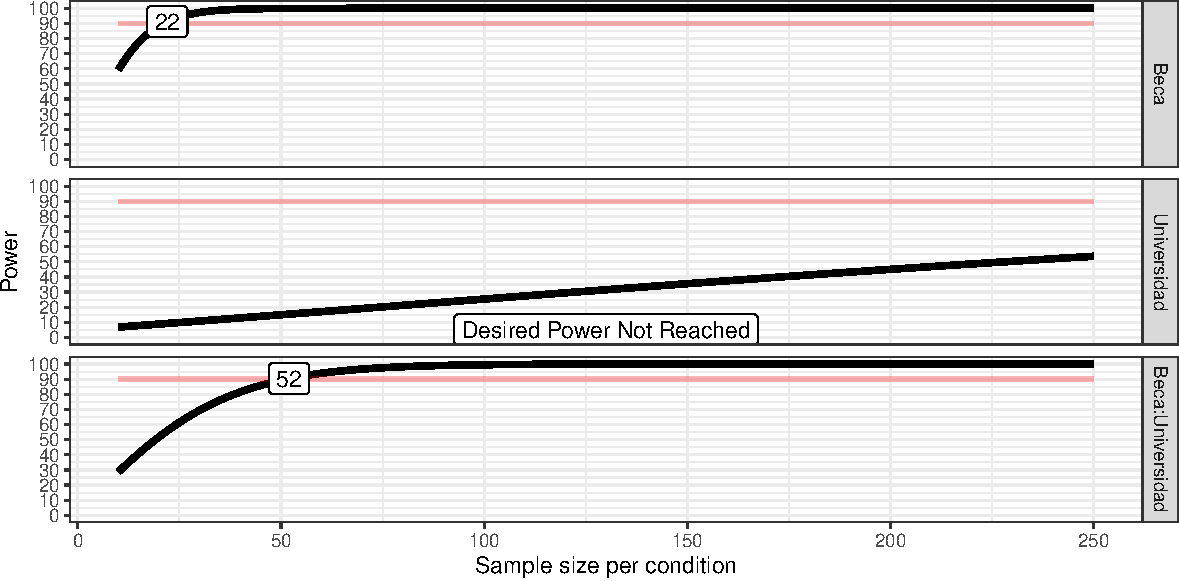
\includegraphics{PowerAnalysisScript_files/figure-latex/fig9-1.pdf}
\caption{\textbf{Figura 9.} Ejemplo de la asociación entre el tamaño de
la muestra y el poder estadístico para un ANOVA 2 \(\times\) 2,
producida con la función \texttt{plot\_power} del paquete
\texttt{Superpower}. Como se puede ver, el poder obtenido según el
tamaño de la muestra es diferente para cada efecto principal o
interacción, pues el tamaño del efecto es diferente en cada caso, por lo
que se requeriría un \emph{n} diferente para alcanzar el mismo poder
estadístico. En este ejemplo, un poder \(1-\beta\) de 0.9 (90\%) se
alcanza para el efecto principal de la \emph{Beca} (\textbf{panel
superior}) con una muestra de apenas unos 24 participantes en cada
combinación de \emph{Beca} y \emph{Universidad} (96 en total), mientras
que ese mismo poder para detectar un efecto principal del tipo de
\emph{Universidad} (\textbf{panel intermedio}) no se logra ni siquiera
con 250 participantes (1000 en total) por cada combinación de
\emph{Beca} y \emph{Universidad} (de hecho, solo se logra al tener cerda
de 600 participantes por condición, ¡o unos 2400 en total!). La
interacción entre \emph{Beca y Universidad} (\textbf{panel inferior}),
logra un poder de 0.9 (90\%) con unos 50 participantes (200 en total)
por cada combinación de \emph{Beca} y \emph{Universidad}.}
\end{figure}

\hypertarget{anova-factorial-de-medidas-repetidas}{%
\subsection{ANOVA factorial de medidas
repetidas}\label{anova-factorial-de-medidas-repetidas}}

En el paquete \texttt{Superpower} el análisis de poder para diseños
factoriales de medidas repetidas es casi idéntico al de medidas
independientes: se deben usar las funciones (1) \texttt{ANOVA\_design}
para especificar las características del diseño para el cual haré el
análisis de poder, y (2) \texttt{ANOVA\_power} y/o \texttt{plot\_power}
para el análisis de poder propiamente dicho.

Sin embargo, hay una diferencia importante: dado que tendremos factores
de medidas repetidas, se debe especificar la correlación entre estos
niveles, \emph{concatenando} los \emph{r} de Pearson con el argumento
\texttt{r} de la función \texttt{ANOVA\_design} (que no habíamos usado).

El orden para ingresar estos coeficientes de correlación (\emph{r} de
Pearson), debe seguir un criterio específico. Este orden, que debe ser
respetado, es equivalente al ``\emph{triángulo superior}'' (resaltado en
\colorbox{yellow}{\textbf{amarillo}}) de una matriz de correlaciones
(\textbf{Tabla 4}).

\begin{table}[H]

\caption{\label{tab:tab4}\textbf{Tabla 4.} Orden para ingresar los coeficientes de una matriz de correlación entre niveles de un estudio 2 $\times$ 2 de medidas repetidas}
\centering
\begin{threeparttable}
\begin{tabular}[t]{>{}lcccc}
\toprule
  & A1 - B1 & A1 - B2 & A2 - B1 & A2 - B2\\
\midrule
\textbf{A1 - B1} & - & \cellcolor{yellow}{\textbf{1}} & \cellcolor{yellow}{\textbf{2}} & \cellcolor{yellow}{\textbf{3}}\\
\textbf{A1 - B2} & 1 & - & \cellcolor{yellow}{\textbf{4}} & \cellcolor{yellow}{\textbf{5}}\\
\textbf{A2 - B1} & 2 & 4 & - & \cellcolor{yellow}{\textbf{6}}\\
\textbf{A2 - B2} & 3 & 5 & 6 & -\\
\bottomrule
\end{tabular}
\begin{tablenotes}
\item \textit{Nota:} 
\item Los números representan el orden en el que deben ser ingresados los coeficientes de correlación en el argumento r de la función ANOVA\_design. Se puede usar en triángulo superior (resaltado en amarillo).
\end{tablenotes}
\end{threeparttable}
\end{table}

\hypertarget{ejemplo-anova-factorial-de-medidas-repetidas-2-times-2}{%
\subsubsection{\texorpdfstring{Ejemplo ANOVA factorial de medidas
repetidas (2 \(\times\)
2)}{Ejemplo ANOVA factorial de medidas repetidas (2 \textbackslash times 2)}}\label{ejemplo-anova-factorial-de-medidas-repetidas-2-times-2}}

Por ejemplo, si tuviéramos un diseño donde medimos la ansiedad de un
grupo de personas tras tomar una tasa de café con cafeína o
descafeinado, en un día laboral y en un día de descanso, tendríamos un
diseño 2 \(\times\) 2 con dos factores de medidas repetidas, cada uno
con dos niveles:

\begin{itemize}
\tightlist
\item
  Factor 1: Cafeína (Sí, No)
\item
  Factor 2: Día laboral (Sí, No)
\end{itemize}

En este caso, la ansiedad de cada participante sería medida cuatro
veces, tras tomar:

\begin{enumerate}
\def\labelenumi{\arabic{enumi}.}
\tightlist
\item
  Café con cafeína en un día laboral (Cafeína Sí; Día laboral Sí).
\item
  Café con cafeína en un día de descanso (Cafeína Sí; Día laboral No).
\item
  Café sin cafeína en un día laboral (Cafeína No; Día laboral Sí).
\item
  Café Sin cafeína en un día de descanso (Cafeína No; Día laboral No).
\end{enumerate}

Lo importante es entonces especificar las correlaciones entre estas
condiciones. Para esto, lo mejor es hacer una matriz de correlaciones
(\textbf{Tabla 5}).

\begin{table}[H]

\caption{\label{tab:tab5}\textbf{Tabla 5.} Matriz de correlación hipotética entre niveles de un estudio 2 $\times$ 2 de medidas repetidas}
\centering
\begin{threeparttable}
\begin{tabular}[t]{lcccc}
\toprule
  & \makecell[c]{Cafeína Sí; \\ Día laboral Sí} & \makecell[c]{Cafeína Sí; \\ Día laboral No} & \makecell[c]{Cafeína No; \\ Día laboral Sí} & \makecell[c]{Cafeína No; \\ Día laboral No}\\
\midrule
Cafeína Sí; 
 Día laboral Sí & \cellcolor[HTML]{c4c4c4}{1} & \cellcolor{yellow}{\textbf{0.384}} & \cellcolor{yellow}{\textbf{0.287}} & \cellcolor{yellow}{\textbf{0.302}}\\
Cafeína Sí; 
 Día laboral No & 0.384 & \cellcolor[HTML]{c4c4c4}{1} & \cellcolor{yellow}{\textbf{0.204}} & \cellcolor{yellow}{\textbf{0.402}}\\
Cafeína No; 
 Día laboral Sí & 0.287 & 0.204 & \cellcolor[HTML]{c4c4c4}{1} & \cellcolor{yellow}{\textbf{0.184}}\\
Cafeína No; 
 Día laboral No & 0.302 & 0.402 & 0.184 & \cellcolor[HTML]{c4c4c4}{1}\\
\bottomrule
\end{tabular}
\begin{tablenotes}
\item \textit{Nota:} 
\item Los coeficientes de correlación resaltados en amarillo (triángulo superior), son los que se deben ingresar en el argumento r de la función ANOVA\_design, siguiendo el orden especificado (e.g. Tabla 4). En gris está resaltada la diagonal de la matriz de correlaciones, que contiene la correlación de cada variable consigo misma.
\end{tablenotes}
\end{threeparttable}
\end{table}

Teniendo esto en cuenta, podemos especificar este diseño en la función
\texttt{ANOVA\_design}, incluyendo los coeficientes de correlación
(\textbf{Table 5}) en el orden descrito (\textbf{Tabla 4}) en el
argumento \texttt{r}. En total, los argumentos incluidos son:

\begin{enumerate}
\def\labelenumi{\arabic{enumi}.}
\item
  \texttt{design}: en este caso, dado que tengo un diseño 2 \(\times\)
  2, donde ambos factores son de medidas repetidas, debo ponerlo como
  \texttt{"2w*2w"}, donde los números representan el número de niveles
  en cada factor, la letra \textbf{w} que ese factor en de medidas
  repetidas (o \emph{intra sujetos}, por lo cual usa la letra
  \textbf{w}, del inglés \emph{within-subjects}).
\item
  \texttt{n}: el número de participantes que espero tener; como mis
  factores son de medidas repetidas o intra-sujetos, lo importante es
  que para cada participante sea se hagan observaciones para cada
  condición (o, dicho de otro modo, por combinación de niveles de mis
  factores; e.g.~(1) tras tomar café con cafeína en un día laboral; (2)
  tras tomar café con cafeína en un día no laboral, etcétera). Como lo
  mencioné anteriormente, a diferencia de otros paquetes y programas,
  \texttt{Superpower} no calcula el \emph{n} por mí, pero me permite
  cambiar el \emph{n} hasta lograr el poder deseado.
\item
  \texttt{mu}: las medias para cada interacción entre los niveles de mis
  factores. En este caso, la media de la ansiedad para participantes al
  tomar (1) café con cafeína en un día laboral, (2) café con cafeína en
  un día no laboral, (3) café descafeinado en un día laboral, y (4) café
  descafeinado en un día no laboral. Estos valores, como antes, deben
  estar \emph{concatenados} usando la función \texttt{c}.
\item
  \texttt{sd}: la desviación estándar para la población (por lo cual es
  un solo valor. En este caso, la desviación estándar de los puntajes de
  ansiedad).
\item
  \texttt{r}: los coeficientes de correlación entre combinaciones de mis
  factores intra-sujetos o de medidas repetidas, en el orden correcto
  (como fue descrito en la \textbf{Tabla 4}).
\item
  \texttt{labelnames} (Opcional): las etiquetas (nombres) de los
  factores y sus niveles. Al igual que con las medias, estas etiquetas
  deben estar concatenadas usando la función \texttt{c}. Como expliqué
  en la sección \protect\hyperlink{ind}{7.4 ANOVA factorial de medidas
  independientes}, para definirlos, se deben poner en el siguiente
  orden:

  \begin{itemize}
  \tightlist
  \item
    Etiqueta del primer factor (en este caso ``Cafeína'')
  \item
    Etiquetas de los niveles de ese factor (en este caso ``Sí'' y
    ``No'')
  \item
    Etiqueta del segundo factor (en este caso ``Día\_laboral'', pues
    estos nombres NO pueden tener espacios).
  \item
    Etiquetas de los niveles de ese factor (en este caso ``Sí'' y
    ``No'').
  \end{itemize}
\end{enumerate}

En este caso, el diseño lo \emph{guardaré} como un objeto llamado
\texttt{disenoW}, y usé la opción \texttt{plot\ =\ TRUE} para asegurarme
de que las medias fueron \emph{concatenadas} en el orden correcto
(\textbf{Figura 10}).

\begin{Shaded}
\begin{Highlighting}[]
\NormalTok{disenoW }\OtherTok{\textless{}{-}} \FunctionTok{ANOVA\_design}\NormalTok{(}\AttributeTok{design =} \StringTok{"2w*2w"}\NormalTok{,}
                        \AttributeTok{n =} \DecValTok{100}\NormalTok{, }\AttributeTok{sd =} \FloatTok{3.5}\NormalTok{, }
                        \AttributeTok{mu =} \FunctionTok{c}\NormalTok{(}\FloatTok{25.1}\NormalTok{, }\FloatTok{21.2}\NormalTok{, }\FloatTok{26.3}\NormalTok{, }\FloatTok{24.2}\NormalTok{), }
\NormalTok{                        r }\OtherTok{\textless{}{-}} \FunctionTok{c}\NormalTok{(}\FloatTok{0.384}\NormalTok{, }\FloatTok{0.287}\NormalTok{, }\FloatTok{0.302}\NormalTok{, }\FloatTok{0.204}\NormalTok{, }\FloatTok{0.402}\NormalTok{, }\FloatTok{0.184}\NormalTok{),}
                        \AttributeTok{labelnames =} \FunctionTok{c}\NormalTok{(}\StringTok{"Cafeína"}\NormalTok{, }\StringTok{"Sí"}\NormalTok{, }\StringTok{"No"}\NormalTok{, }\StringTok{"Día\_laboral"}\NormalTok{, }\StringTok{"Sí"}\NormalTok{, }\StringTok{"No"}\NormalTok{),}
                        \AttributeTok{plot =} \ConstantTok{TRUE}\NormalTok{)}
\end{Highlighting}
\end{Shaded}

\begin{figure}
\centering
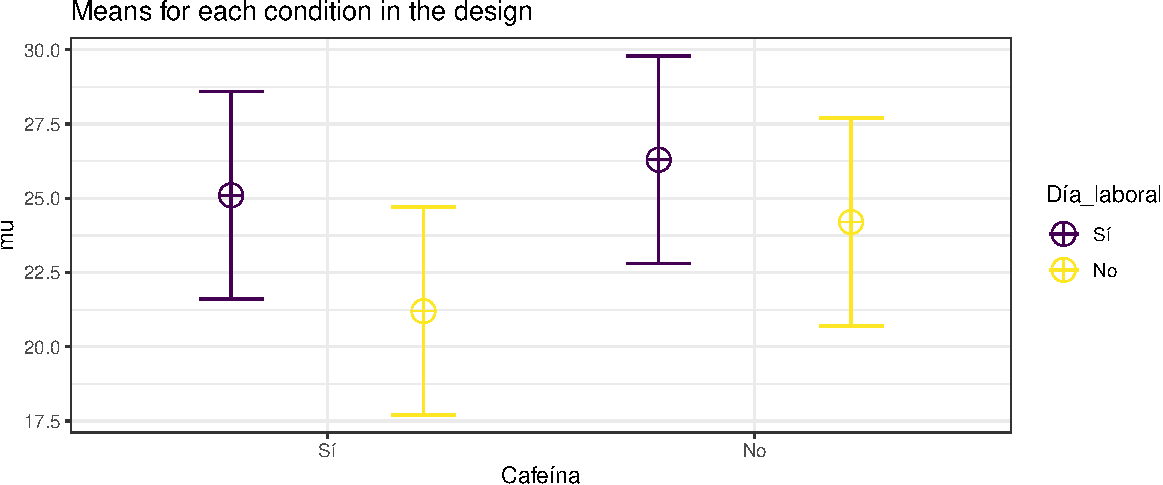
\includegraphics{PowerAnalysisScript_files/figure-latex/fig10-1.pdf}
\caption{\textbf{Figura 10.} Ejemplo de la distribución de medias
marginales estimadas y sus intervalos de confianza para el diseño
definido con la función \texttt{ANOVA\_design}, al incluir el argumento
\texttt{plot\ =\ TRUE}. Esto es muy útil para estar seguro de que las
medias fueron \emph{concatenadas} en el orden correcto.}
\end{figure}

Del mismo modo, para asegurarme de que los coeficientes de correlación
fueron \emph{concatenados} en el orden correcto, puedo pedir una matriz
de correlaciones usando el nombre del objeto que contiene el diseño (en
este caso \texttt{disenoW}) y agregando \texttt{\$cor\_mat}, y confirmar
que los valores y su orden corresponden con la matriz original (en este
caso, en la \textbf{Tabla 5}).

\begin{Shaded}
\begin{Highlighting}[]
\NormalTok{disenoW}\SpecialCharTok{$}\NormalTok{cor\_mat}
\end{Highlighting}
\end{Shaded}

\begin{verbatim}
##       Sí_Sí Sí_No No_Sí No_No
## Sí_Sí 1.000 0.384 0.287 0.302
## Sí_No 0.384 1.000 0.204 0.402
## No_Sí 0.287 0.204 1.000 0.184
## No_No 0.302 0.402 0.184 1.000
\end{verbatim}

Una vez definido el diseño y las características de los datos
(\emph{``guardando''} este diseño en un objeto que llamé
\texttt{disenoW}), puedo ver el poder que obtendría con esos 100
participantes por cada combinación de \emph{Cafeína} y \emph{Día
laboral}, con la función \texttt{ANOVA\_power}, de la misma manera que
lo haría para un diseño de medidas independientes.

\begin{Shaded}
\begin{Highlighting}[]
\FunctionTok{ANOVA\_power}\NormalTok{(disenoW,}
            \AttributeTok{alpha\_level =} \FloatTok{0.05}\NormalTok{,}
            \AttributeTok{p\_adjust =} \StringTok{"holm"}\NormalTok{,}
            \AttributeTok{seed =} \DecValTok{1685}\NormalTok{,}
            \AttributeTok{nsims =} \DecValTok{1000}\NormalTok{)}
\end{Highlighting}
\end{Shaded}

\begin{verbatim}
## Power and Effect sizes for ANOVA tests
##                           power effect_size
## anova_Cafeína             100.0      0.3469
## anova_Día_laboral         100.0      0.4795
## anova_Cafeína:Día_laboral  89.9      0.1029
## 
## Power and Effect sizes for pairwise comparisons (t-tests)
##                                                       power effect_size
## p_Cafeína_Sí_Día_laboral_Sí_Cafeína_Sí_Día_laboral_No 100.0     -1.0095
## p_Cafeína_Sí_Día_laboral_Sí_Cafeína_No_Día_laboral_Sí  76.1      0.2875
## p_Cafeína_Sí_Día_laboral_Sí_Cafeína_No_Día_laboral_No  55.0     -0.2210
## p_Cafeína_Sí_Día_laboral_No_Cafeína_No_Día_laboral_Sí 100.0      1.1612
## p_Cafeína_Sí_Día_laboral_No_Cafeína_No_Día_laboral_No 100.0      0.7888
## p_Cafeína_No_Día_laboral_Sí_Cafeína_No_Día_laboral_No  98.4     -0.4731
\end{verbatim}

Como se puede ver, el poder estadístico para detectar posibles efectos
de \emph{Cafeína} (\(1-\beta\) = 100\%), \emph{Día laboral} (\(1-\beta\)
= 100\%), y la interacción \emph{Cafeína} \(\times\) Día laboral
(\(1-\beta\) = 89.9\%), es más que suficiente con 100 participantes por
condición (y casi el nivel deseado para la interacción), pues los
tamaños del efecto estimado, son relativamente grandes ( \(\eta_p^2\) =
0.3469, 0.4795, y 0.1029, respectivamente).

Del mismo modo, un \emph{n} de 100 participantes por condición, da un
poder suficiente (\(1-\beta\) \textgreater{} 0.9) para detectar casi
todas las diferencias según fueron estimadas, excepto: (1) la
diferencia, tal cual fue estimada, entre los niveles de ansiedad tras
tomar café con cafeína vs café descafeinado en un día laboral
(\(1-\beta\) = 76.1\%); y (2), la diferencia entre los niveles de
ansiedad tras tomar café con cafeína en un día laboral, vs café
descafeinado en un día no laboral (\(1-\beta\) = 55\%), que por supuesto
tienen los tamaños de efecto más pequeños (más cercanos a 0),
independientemente de su dirección (\emph{d} = 0.2875, y -0.2210,
respectivamente).

Sin embargo, para estimar el tamaño de muestra suficiente, puedo como
antes usar la función \texttt{plot\_power} (\textbf{Figura 11}),
definiendo tanto el n mínimo (\texttt{min\_n}) y el n máximo
(\texttt{max\_n}) que deseo incluir en mi figura:

\begin{Shaded}
\begin{Highlighting}[]
\FunctionTok{plot\_power}\NormalTok{(disenoW, }
           \AttributeTok{min\_n =} \DecValTok{5}\NormalTok{, }
           \AttributeTok{max\_n =} \DecValTok{100}\NormalTok{, }
           \AttributeTok{plot =} \ConstantTok{TRUE}\NormalTok{)}
\end{Highlighting}
\end{Shaded}

\begin{figure}
\centering
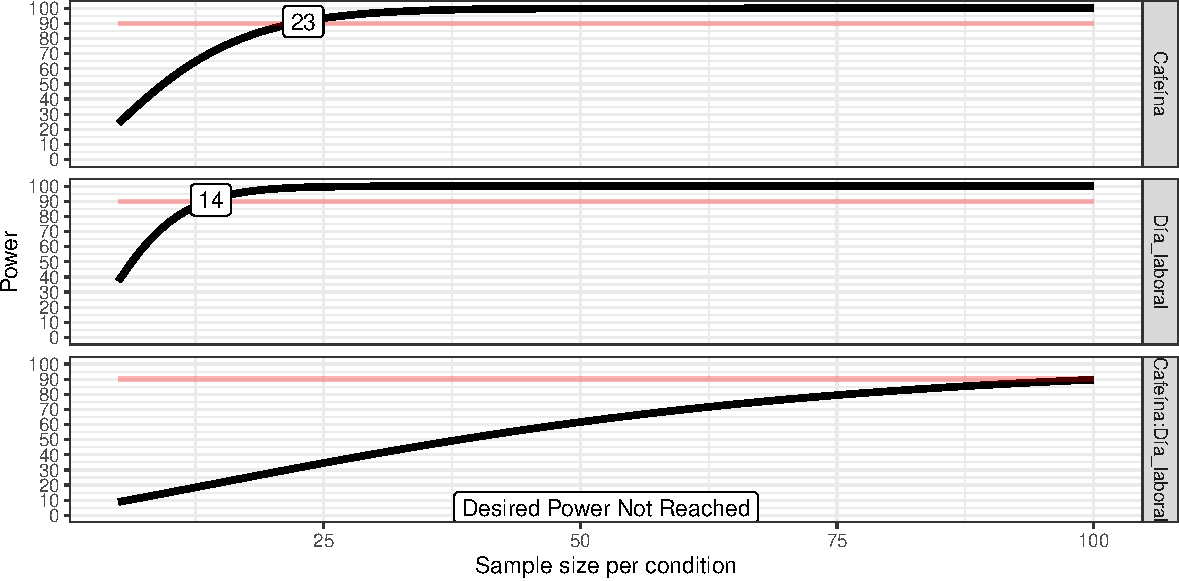
\includegraphics{PowerAnalysisScript_files/figure-latex/fig11-1.pdf}
\caption{\textbf{Figura 11.} Ejemplo de la asociación entre el tamaño de
la muestra y el poder estadístico para un ANOVA 2 \(\times\) 2,
producida con la función \texttt{plot\_power} del paquete
\texttt{Superpower}. Como se puede ver, el poder obtenido según el
tamaño de la muestra es diferente para cada efecto principal o
interacción, pues el tamaño del efecto es diferente en cada caso, por lo
que se requeriría un \emph{n} diferente para alcanzar el mismo poder
estadístico. En este ejemplo, un poder \(1-\beta\) de 0.9 (90\%) se
alcanza para el efecto principal de la \emph{Cafeína} (\textbf{panel
superior}) con una muestra de apenas unos 20 participantes, mientras que
ese mismo poder para detectar un efecto principal del tipo de \emph{Día
laboral} (\textbf{panel intermedio}) se logra con alrededor de 13
participantes, y la interacción entre \emph{Cafeína y Día laboral}
(\textbf{panel inferior}), logra un poder de 0.9 (90\%) con unos 100
participantes. Si mi interés principal es la interacción entre estas
variables, debo entonces usar una muestra de unos 100 participantes, a
los cuales se les medirá la ansiedad en las cuatro condiciones en cada
condición.}
\end{figure}

\hypertarget{anova-factorial-mixto}{%
\subsection{ANOVA factorial mixto}\label{anova-factorial-mixto}}

Si se entiende cómo hacer análisis de poder para diseños factoriales de
medidas repetidas, y de medidas independientes en el paquete
\texttt{Superpower}, hacer análisis para diseños mixtos es sencillo.

Básicamente, un diseño mixto es cuando tenemos factores (variables
independientes nominales) tanto de medidas repetidas como
independientes. Como tal, requiere combinar elementos de los análisis de
poder de medidas independientes, con los de medidas repetidas, y se hace
con las mismas funciones ya usadas: (1) \texttt{ANOVA\_design} para
especificar las características del diseño para el cual haré el análisis
de poder, y (2) \texttt{ANOVA\_power} y/o \texttt{plot\_power} para el
análisis de poder propiamente dicho.

Las diferencias son que, al especificar el diseño con la función
\texttt{ANOVA\_design} (argumento \texttt{design}), se debe especificar
que hay niveles intra-sujetos (de medidas repetidas, que en el paquete
se designado como \textbf{w}, del inglés \emph{within-subjects}) y
entre-sujetos (medidas independientes, \textbf{b}, del inglés
\emph{between-subjects}).

Adicionalmente, tenemos que especificar la correlación entre los niveles
de factores intra-sujeto (tal cual como lo hicimos para diseños de
medidas repetidas), pero no para factores de medidas independientes,
pues en este caso se asume siempre que la correlación es 0\footnote{Por
  esto al hacer análisis de medidas independientes no se especifica
  ninguna correlación.}. De este modo, el número de coeficientes de
correlación que debemos especificar (en el argumento \texttt{r} de la
función \texttt{ANOVA\_design}) es menor al de diseños equivalentes de
medidas repetidas.

\hypertarget{ejemplo-anova-factorial-mixto-2-times-2}{%
\subsubsection{\texorpdfstring{Ejemplo ANOVA factorial mixto (2
\(\times\)
2)}{Ejemplo ANOVA factorial mixto (2 \textbackslash times 2)}}\label{ejemplo-anova-factorial-mixto-2-times-2}}

Por ejemplo, si quisiera medir qué tanto un ruido insoportable (por
ejemplo, el sonido de la \emph{fresa} de un odontólogo afecta el
desempeño de jugadores aficionados de ajedrez\footnote{Es solamente un
  ejemplo. Jamás pensaría en torturar a jugadores de ajedrez, ni a
  nadie, sometiéndolo a semejante tortura solo por curiosidad
  ``científica''.}, en términos de partidas ganadas sobre un total de 20
partidas jugadas, y quisiera saber si este efecto es diferente en
personas según si son odontólogos o no, tendría un diseño mixto 2
\(\times\) 2, pues mis factores serían:

\begin{enumerate}
\def\labelenumi{\arabic{enumi}.}
\tightlist
\item
  Factor 1 (medidas independientes): Profesión (Odontólogo, Otro)
\item
  Factor 2 (medidas repetidas): Ruido (NO, Sí)
\end{enumerate}

En este caso, tendría que someter a cada uno de mis participantes,
odontólogos o no, a dos rondas de 20 juegos de ajedrez (una ronda con, y
otra sin presencia del ruido).

Como siempre, con la información clara, puedo definir los argumentos del
diseño, con la función \texttt{ANOVA\_design}, teniendo en cuenta que,
como esta vez solo tengo un factor de medidas repetidas (\emph{Ruido}),
y este tiene solo dos niveles (sí, No), solo debo especificar ese
coeficiente de correlación.

En este caso, el diseño lo \emph{``guardaré''} como un objeto llamado
\texttt{disenoM}, y usé la opción \texttt{plot\ =\ TRUE} para asegurarme
de que las medias fueron concatenadas en el orden correcto.

Como se puede ver en el código a continuación, y en la \textbf{Figura
12}, según mis datos (inventados), tanto odontólogos como no odontólogos
ganan en promedio cerca de 12 partidas de 20 jugadas (\(\approx\) 60\%),
cuando las juegan sin ruido (en morado), pero el desempeño de personas
con profesiones distintas a la odontología se ve muy afectado al jugar
las partidas en presencia del ruido.

Dado que no sería fácil conseguir voluntarios para someterse a jugar, en
total, 40 partidas de ajedrez, de las cuales 20 se jugarían con un ruido
insoportable, pero que también espero un tamaño de efecto grande, voy a
hacer el cálculo solo con 10 participantes por grupo (10 odontólogos, 10
no odontólogos).

\begin{Shaded}
\begin{Highlighting}[]
\NormalTok{disenoM }\OtherTok{\textless{}{-}} \FunctionTok{ANOVA\_design}\NormalTok{(}\AttributeTok{design =} \StringTok{"2b*2w"}\NormalTok{,}
                        \AttributeTok{n =} \DecValTok{10}\NormalTok{, }
                        \AttributeTok{mu =} \FunctionTok{c}\NormalTok{(}\DecValTok{13}\NormalTok{, }\DecValTok{12}\NormalTok{, }\DecValTok{14}\NormalTok{, }\DecValTok{6}\NormalTok{),}
                        \AttributeTok{sd =} \FloatTok{3.12}\NormalTok{,}
                        \AttributeTok{r =} \FloatTok{0.3}\NormalTok{,}
                        \AttributeTok{labelnames =} \FunctionTok{c}\NormalTok{(}\StringTok{"Profesión"}\NormalTok{, }\StringTok{"Odontólogo"}\NormalTok{, }\StringTok{"Otro"}\NormalTok{, }\StringTok{"Ruido"}\NormalTok{, }\StringTok{"No"}\NormalTok{, }\StringTok{"Sí"}\NormalTok{),}
                        \AttributeTok{plot =} \ConstantTok{TRUE}\NormalTok{)}
\end{Highlighting}
\end{Shaded}

\begin{figure}
\centering
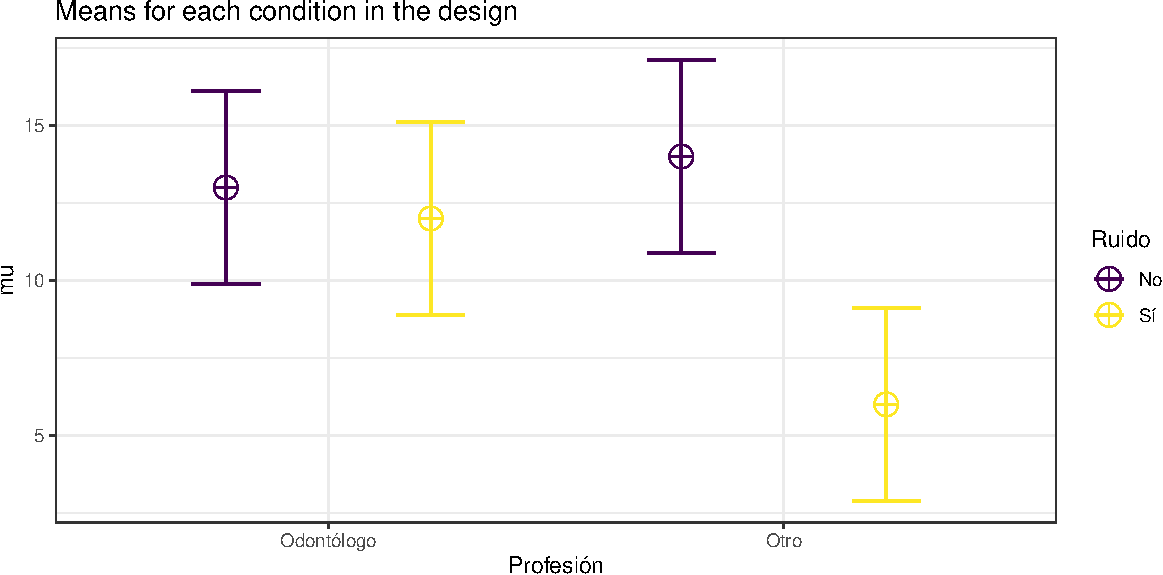
\includegraphics{PowerAnalysisScript_files/figure-latex/fig12-1.pdf}
\caption{\textbf{Figura 12.} Ejemplo de la distribución de medias
marginales estimadas y sus intervalos de confianza para el diseño
definido con la función \texttt{ANOVA\_design}, al incluir el argumento
\texttt{plot\ =\ TRUE}. Esto es muy útil para estar seguro de que las
medias fueron \emph{concatenadas} en el orden correcto.}
\end{figure}

También, como siempre, puedo pedir una matriz de correlaciones usando el
nombre del objeto que contiene el diseño (en este caso \texttt{disenoM}
y agregando \texttt{\$cor\_mat}) para asegurarme de que los coeficientes
de correlación están en el orden correcto.

\begin{Shaded}
\begin{Highlighting}[]
\NormalTok{disenoM}\SpecialCharTok{$}\NormalTok{cor\_mat}
\end{Highlighting}
\end{Shaded}

\begin{verbatim}
##               Odontólogo_No Odontólogo_Sí Otro_No Otro_Sí
## Odontólogo_No           1.0           0.3     0.0     0.0
## Odontólogo_Sí           0.3           1.0     0.0     0.0
## Otro_No                 0.0           0.0     1.0     0.3
## Otro_Sí                 0.0           0.0     0.3     1.0
\end{verbatim}

Definido el diseño y las características de los datos (que
\emph{``guardé''} en un objeto que llamé \texttt{disenoM}), puedo ver el
poder que obtendría con esos 10 participantes por grupo, con la función
\texttt{ANOVA\_power}, de la misma manera que lo haría para diseños de
medidas independientes o repetidas.

\begin{Shaded}
\begin{Highlighting}[]
\FunctionTok{ANOVA\_power}\NormalTok{(disenoM,}
            \AttributeTok{alpha\_level =} \FloatTok{0.05}\NormalTok{,}
            \AttributeTok{p\_adjust =} \StringTok{"holm"}\NormalTok{,}
            \AttributeTok{seed =} \DecValTok{1985}\NormalTok{,}
            \AttributeTok{nsims =} \DecValTok{1000}\NormalTok{)}
\end{Highlighting}
\end{Shaded}

\begin{verbatim}
## Power and Effect sizes for ANOVA tests
##                       power effect_size
## anova_Profesión        57.2      0.2368
## anova_Ruido           100.0      0.6248
## anova_Profesión:Ruido  97.2      0.5070
## 
## Power and Effect sizes for pairwise comparisons (t-tests)
##                                                               power effect_size
## p_Profesión_Odontólogo_Ruido_No_Profesión_Odontólogo_Ruido_Sí   5.0     -0.2934
## p_Profesión_Odontólogo_Ruido_No_Profesión_Otro_Ruido_No         6.1      0.3345
## p_Profesión_Odontólogo_Ruido_No_Profesión_Otro_Ruido_Sí        98.8     -2.3496
## p_Profesión_Odontólogo_Ruido_Sí_Profesión_Otro_Ruido_No        12.6      0.6522
## p_Profesión_Odontólogo_Ruido_Sí_Profesión_Otro_Ruido_Sí        93.9     -2.0133
## p_Profesión_Otro_Ruido_No_Profesión_Otro_Ruido_Sí              99.8     -2.3956
\end{verbatim}

Como se puede ver, el poder estadístico para detectar posibles efectos
de \emph{Profesión} (\(1-\beta\) = 57.2\%) es algo bajo con solo 10
participantes por grupo, mientras que el poder para detectar un efecto
de la condición de \emph{Ruido} (\(1-\beta\) = 100\%), y la interacción
\emph{Profesión} × \emph{Ruido} (\(1-\beta\) = 97.2\%), es más que
suficiente. Esto se da porque los tamaños de efecto son bastante grandes
(\(\eta_p^2\) = 0.2368, 0.6248, y 0.5070, respectivamente), por lo cual
nunca será necesaria una muestra demasiado grande (ni siquiera en el
caso de la \emph{Profesión}, como lo sugiere el hecho de que con apenas
10 participantes por grupo se obtenga un poder no muy lejano al
deseado).

El poder para detectar comparaciones \emph{post-hoc} es, sin embargo,
muy bajo en varios casos. Solamente al comparar a los no odontólogos
jugando con ruido vs odontólogos jugando con o sin ruido, o esos mismo
no odontólogos jugando sin ruido, se logra un poder suficiente (lo que
no es una sorpresa si se tienen en cuenta las medias esperadas;
\textbf{Figura 11}).

Sin embargo, para estimar el tamaño de muestra suficiente, puedo como
antes usar la función \texttt{plot\_power} (\textbf{Figura 13}),
definiendo tanto el \emph{n} mínimo (\texttt{min\_n}) y el \emph{n}
máximo (\texttt{max\_n}) que deseo incluir en mi figura:

\begin{Shaded}
\begin{Highlighting}[]
\FunctionTok{plot\_power}\NormalTok{(disenoM,}
           \AttributeTok{min\_n =} \DecValTok{1}\NormalTok{,}
           \AttributeTok{max\_n =} \DecValTok{30}\NormalTok{,}
           \AttributeTok{plot =} \ConstantTok{TRUE}\NormalTok{)}
\end{Highlighting}
\end{Shaded}

\begin{figure}
\centering
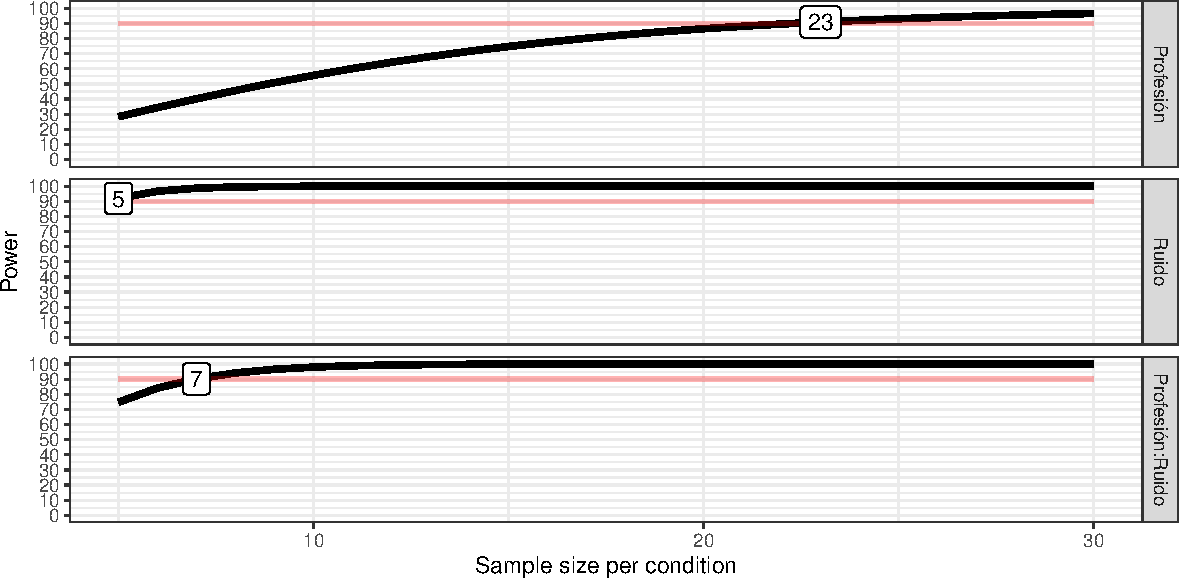
\includegraphics{PowerAnalysisScript_files/figure-latex/fig13-1.pdf}
\caption{\textbf{Figura 13.} Ejemplo de la asociación entre el tamaño de
la muestra y el poder estadístico para un ANOVA 2 \(\times\) 2 mixto,
producida con la función \texttt{plot\_power} del paquete
\texttt{Superpower}. Como se puede ver, el poder obtenido según el
tamaño de la muestra es diferente para cada efecto principal o
interacción, pues el tamaño del efecto es diferente en cada caso, por lo
que se requeriría un \emph{n} diferente para alcanzar el mismo poder
estadístico. En este ejemplo, un poder \(1-\beta\) de 0.9 (90\%) se
alcanza para el efecto principal de la \emph{Profesión} (\textbf{panel
superior}) con una muestra de apenas unos 18 participantes por grupo,
mientras que ese mismo poder para detectar un efecto principal del tipo
de \emph{Ruido} (\textbf{panel intermedio}) se logra con al apenas unos
8 participantes por grupo, y la interacción entre \emph{Profesión y
Ruido} (\textbf{panel inferior}), logra un poder de 0.9 (90\%) con unos
6 participantes por grupo. Si me interesan tanto los efectos principales
como la interacción entre estas variables, debo entonces usar una
muestra de unos 18 participantes por grupo (18 odontólogos y 18 no
odontólogos, para un total de 36 participantes), a los cuales se les
medirá el número de partidas de ajedrez ganadas de 20 jugadas, en las
dos condiciones de ruido.}
\end{figure}

\hypertarget{extra-cuxf3mo-estima-superpower-el-poder-estaduxedstico-con-base-en-simulaciones-de-bases-de-datos}{%
\subsection{\texorpdfstring{Extra: Cómo estima \texttt{Superpower} el
poder estadístico con base en simulaciones de bases de
datos}{Extra: Cómo estima Superpower el poder estadístico con base en simulaciones de bases de datos}}\label{extra-cuxf3mo-estima-superpower-el-poder-estaduxedstico-con-base-en-simulaciones-de-bases-de-datos}}

El poder, como lo mencioné en la sección \protect\hyperlink{power}{1.1
¿Qué es potencia o poder estadístico?}, es la probabilidad de detectar,
como significativo (es decir, con un \(p < \alpha\), que típicamente se
establece en 0.05), un efecto, cuando este existe. Si aspiramos a tener
un poder \(1-\beta\) de 0.9 (90\%), en el 90\% de los casos deberíamos
encontrar un \(p < \alpha\) (es decir, significativo).

Como lo mencioné brevemente antes, la función \texttt{ANOVA\_power}
simula un número de bases de datos (que definimos con el argumento
\texttt{nsims}, para el que yo en todos los ejemplos he usado 1000
simulaciones). Estas bases de datos tienden a seguir las características
que definí al usar la función \texttt{ANOVA\_design}, pero varían
aleatoriamente, como sucedería con datos reales, que difícilmente se
ajustan exactamente a lo esperado.

Entonces, si al usar la función \texttt{ANOVA\_power} pido 1000
simulaciones (\texttt{nsims\ =\ 1000}), se crearán 1000 bases de datos
aleatorias. Para cada una se hace el ANOVA y las comparaciones
\emph{post-hoc}, y sus valores \emph{p}. Entonces, se mira la
probabilidad para cada uno de esos resultados de obtener un valor
significativo (dado el \(\alpha\) definido con el argumento
\texttt{alpha\_level}, que suele definirse en 0.05). En otras palabras,
¿en cuántas de esas 1000 simulaciones se obtuvo un resultado
significativo? Ese porcentaje, es el poder calculado empíricamente.

Ahora, ¿cuál es la distribución de los valores \emph{p} para cada efecto
principal, interacción, o comparación \emph{post-hoc}? Por suerte,
\texttt{Superpower} tiene opciones para ver esto gráficamente.

Si yo \emph{``guardo''} cualquier análisis de poder con base en
simulaciones creado con la función \texttt{ANOVA\_power}, puedo usar el
nombre del objeto en el que grabé ese análisis de poder, y agregar
\texttt{\$plot1} para ver la distribución de los valores \emph{p} para
efectos principales e interacciones, o \texttt{\$plot2} para
comparaciones \emph{post-hoc}.

Por ejemplo, si \emph{``guardo''} una de las simulaciones hechas (en
este caso, usaré la simulación creada para el ANOVA factorial mixto), en
un objeto, que ahora llamaré \texttt{simM}:

\begin{Shaded}
\begin{Highlighting}[]
\NormalTok{simM }\OtherTok{\textless{}{-}} \FunctionTok{ANOVA\_power}\NormalTok{(disenoM,}
                    \AttributeTok{alpha\_level =} \FloatTok{0.05}\NormalTok{,}
                    \AttributeTok{p\_adjust =} \StringTok{"holm"}\NormalTok{,}
                    \AttributeTok{seed =} \DecValTok{1985}\NormalTok{,}
                    \AttributeTok{nsims =} \DecValTok{1000}\NormalTok{)}
\end{Highlighting}
\end{Shaded}

\begin{verbatim}
## Power and Effect sizes for ANOVA tests
##                       power effect_size
## anova_Profesión        57.2      0.2368
## anova_Ruido           100.0      0.6248
## anova_Profesión:Ruido  97.2      0.5070
## 
## Power and Effect sizes for pairwise comparisons (t-tests)
##                                                               power effect_size
## p_Profesión_Odontólogo_Ruido_No_Profesión_Odontólogo_Ruido_Sí   5.0     -0.2934
## p_Profesión_Odontólogo_Ruido_No_Profesión_Otro_Ruido_No         6.1      0.3345
## p_Profesión_Odontólogo_Ruido_No_Profesión_Otro_Ruido_Sí        98.8     -2.3496
## p_Profesión_Odontólogo_Ruido_Sí_Profesión_Otro_Ruido_No        12.6      0.6522
## p_Profesión_Odontólogo_Ruido_Sí_Profesión_Otro_Ruido_Sí        93.9     -2.0133
## p_Profesión_Otro_Ruido_No_Profesión_Otro_Ruido_Sí              99.8     -2.3956
## 
## 
## Within-Subject Factors Included: Check MANOVA Results
\end{verbatim}

Puedo ver a distribución de los valores \emph{p} para efectos
principales e interacciones (\textbf{Figura 14}) con el comando:

\begin{Shaded}
\begin{Highlighting}[]
\NormalTok{simM}\SpecialCharTok{$}\NormalTok{plot1}
\end{Highlighting}
\end{Shaded}

Que produce:

\begin{figure}
\centering
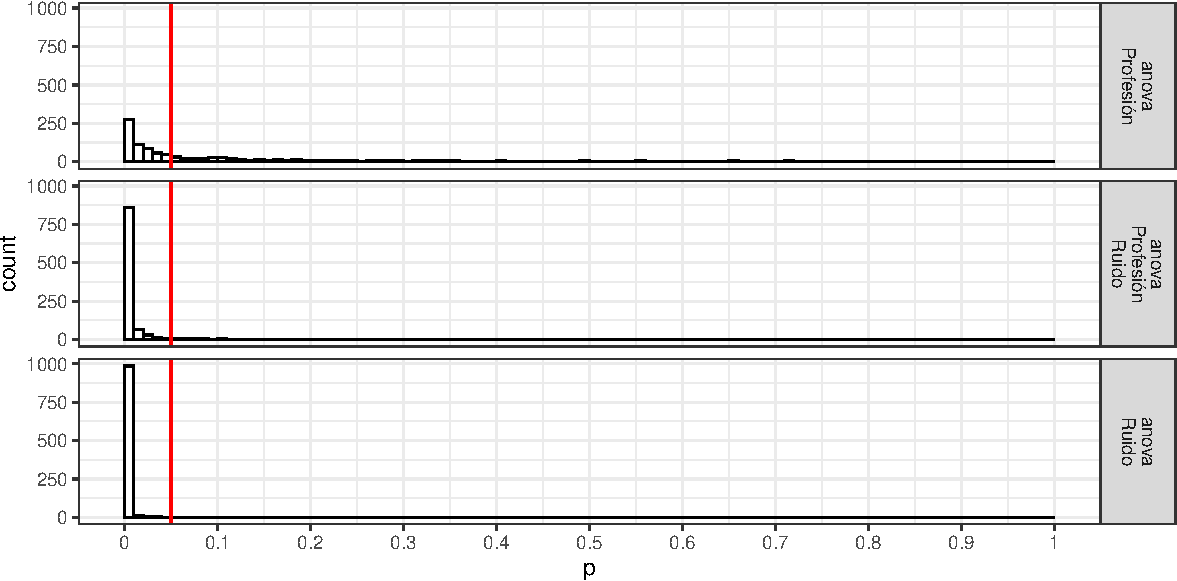
\includegraphics{PowerAnalysisScript_files/figure-latex/unnamed-chunk-29-1.pdf}
\caption{\textbf{Figura 14.} Ejemplo de distribución (histograma) de
valores \emph{p} para efectos principales e interacciones, producto de
1000 simulaciones hechas con la función \texttt{ANOVA\_power} del
paquete \texttt{Superpower}. La línea roja determina el nivel de
significación estadística (\(\alpha\)) definido (en este caso, el típico
0.05).}
\end{figure}

O la distribución de los valores \emph{p} para las comparaciones
\emph{post-hoc} (\textbf{Figura 14}) con el comando:

\begin{Shaded}
\begin{Highlighting}[]
\NormalTok{simM}\SpecialCharTok{$}\NormalTok{plot2}
\end{Highlighting}
\end{Shaded}

Que produce:

\begin{figure}
\centering
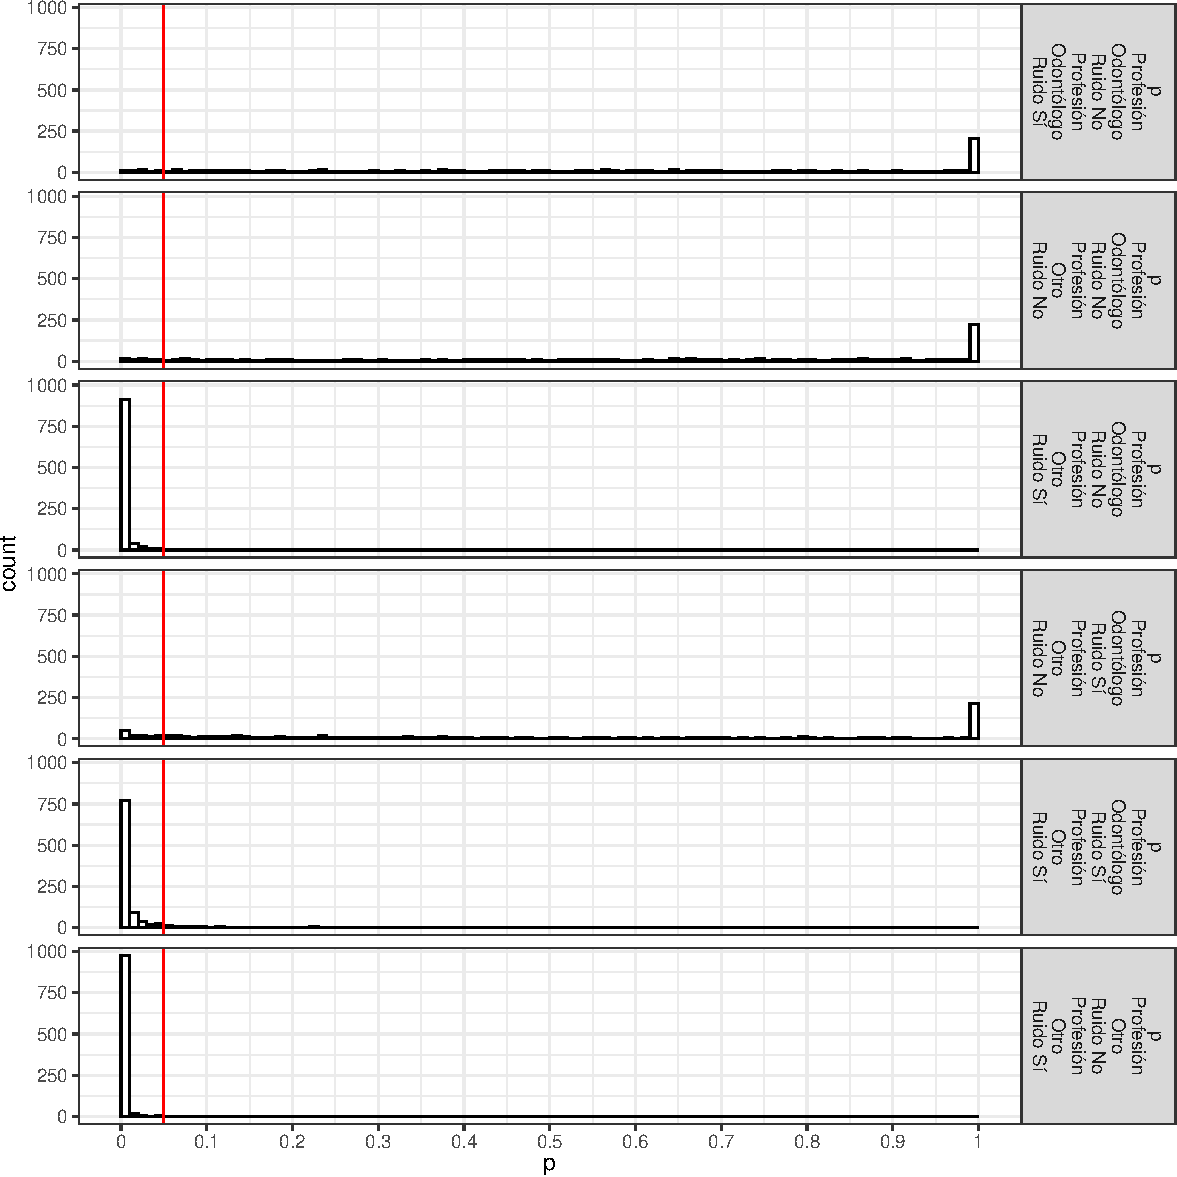
\includegraphics{PowerAnalysisScript_files/figure-latex/unnamed-chunk-31-1.pdf}
\caption{\textbf{Figura 14.} Ejemplo de distribución (histograma) de
valores \emph{p} para comparaciones \emph{post-hoc}, producto de 1000
simulaciones hechas con la función \texttt{ANOVA\_power} del paquete
\texttt{Superpower}. Al contrario de las distribuciones de valores
\emph{p} para ejectos principales e interacciones (\textbf{Figura 13}),
que tienen una tendencia clara, para comparaciones \emph{post-hoc} como
estas la distribución puede verse extraña (aparecen, de repente, muchos
unos) para comparaciones de efectos de tamaño pequeño, y que por ende
tienen bajo poder, dada la corrección solicitada de
\emph{Holm-Bonferroni}. La línea roja determina el nivel de
significación estadística (\(\alpha\)) definido (en este caso, el típico
0.05).}
\end{figure}

\begin{center}\rule{0.5\linewidth}{0.5pt}\end{center}

\hypertarget{refs}{%
\section{Referencias}\label{refs}}

\hypertarget{refs}{}
\begin{CSLReferences}{1}{0}
\leavevmode\vadjust pre{\hypertarget{ref-albersWhenPowerAnalyses2018}{}}%
Albers, C., \& Lakens, D. (2018). When power analyses based on pilot
data are biased: {Inaccurate} effect size estimators and follow-up bias.
\emph{Journal of Experimental Social Psychology}, \emph{74}, 187--195.
\url{https://doi.org/10.1016/j.jesp.2017.09.004}

\leavevmode\vadjust pre{\hypertarget{ref-baker500ScientistsLift2016}{}}%
Baker, M. (2016). 1,500 scientists lift the lid on reproducibility.
\emph{Nature News}, \emph{533}(7604), 452.
\url{https://doi.org/10.1038/533452a}

\leavevmode\vadjust pre{\hypertarget{ref-benjaminRedefineStatisticalSignificance2018}{}}%
Benjamin, D. J., Berger, J. O., Johannesson, M., Nosek, B. A.,
Wagenmakers, E.-J., Berk, R., Bollen, K. A., Brembs, B., Brown, L.,
Camerer, C., Cesarini, D., Chambers, C. D., Clyde, M., Cook, T. D., De
Boeck, P., Dienes, Z., Dreber, A., Easwaran, K., Efferson, C., \ldots{}
Johnson, V. E. (2018). Redefine statistical significance. \emph{Nature
Human Behaviour}, \emph{2}(1), 6--10.
\url{https://doi.org/10.1038/s41562-017-0189-z}

\leavevmode\vadjust pre{\hypertarget{ref-blakesleyComparisonsMethodsMultiple2009}{}}%
Blakesley, R. E., Mazumdar, S., Dew, M. A., Houck, P. R., Tang, G.,
Reynolds III, C. F., \& Butters, M. A. (2009). Comparisons of methods
for multiple hypothesis testing in neuropsychological research.
\emph{Neuropsychology}, \emph{23}(2), 255--264.
\url{https://doi.org/10.1037/a0012850}

\leavevmode\vadjust pre{\hypertarget{ref-bonferroniTeoriaStatisticaClassi1936}{}}%
Bonferroni, C. E. (1936). Teoria statistica delle classi e calcolo delle
probabilit{à}. \emph{Pubblicazioni Del R Istituto Superiore Di Scienze
Economiche e Commerciali Di Firenze}.

\leavevmode\vadjust pre{\hypertarget{ref-buttonPowerFailureWhy2013}{}}%
Button, K. S., Ioannidis, J. P. A., Mokrysz, C., Nosek, B. A., Flint,
J., Robinson, E. S. J., \& Munafò, M. R. (2013). Power failure: Why
small sample size undermines the reliability of neuroscience.
\emph{Nature Reviews Neuroscience}, \emph{14}(5), 365--376.
\url{https://doi.org/10.1038/nrn3475}

\leavevmode\vadjust pre{\hypertarget{ref-caldwellPowerAnalysisSuperpower2020}{}}%
Caldwell, A. R., \& Lakens, D. (2020). \emph{Power {Analysis} with
{Superpower}}. https://aaroncaldwell.us/SuperpowerBook/.

\leavevmode\vadjust pre{\hypertarget{ref-caldwellSuperpowerSimulationBasedPower2020}{}}%
Caldwell, A. R., Lakens, D., DeBruine, L., \& Love, J. (2020).
\emph{Superpower: {Simulation}-{Based Power Analysis} for {Factorial
Designs}}.

\leavevmode\vadjust pre{\hypertarget{ref-champelyPwrBasicFunctions2020}{}}%
Champely, S., Ekstrom, C., Dalgaard, P., Gill, J., Weibelzahl, S.,
Anandkumar, A., Ford, C., Volcic, R., \& Rosario, H. D. (2020).
\emph{Pwr: {Basic Functions} for {Power Analysis}}.

\leavevmode\vadjust pre{\hypertarget{ref-chathamPlannedContrastsOverview1999}{}}%
Chatham, K. (1999). \emph{Planned {Contrasts}: {An Overview} of
{Comparison Methods}}.

\leavevmode\vadjust pre{\hypertarget{ref-cohenStatisticalPowerAnalysis1988}{}}%
Cohen, J. (1988). \emph{Statistical power analysis for the behavioral
sciences} (2nd ed.). {Erlbaum}.

\leavevmode\vadjust pre{\hypertarget{ref-cohenPowerPrimer1992}{}}%
Cohen, J. (1992). A power primer. \emph{Psychological Bulletin},
\emph{112}(1), 155--159.
\url{https://doi.org/10.1037/0033-2909.112.1.155}

\leavevmode\vadjust pre{\hypertarget{ref-correaScriptsVideo2020}{}}%
Correa, J. C. (2020). Scripts en {R} {[}{Video}{]}. In \emph{YouTube}.
https://www.youtube.com/watch?v=ejQ0BS2gVJI.

\leavevmode\vadjust pre{\hypertarget{ref-correllAvoidCohenSmall2020}{}}%
Correll, J., Mellinger, C., McClelland, G. H., \& Judd, C. M. (2020).
Avoid {Cohen}'s {``{Small},''} {``{Medium},''} and {``{Large}''} for
{Power Analysis}. \emph{Trends in Cognitive Sciences}, \emph{24}(3),
200--207. \url{https://doi.org/10.1016/j.tics.2019.12.009}

\leavevmode\vadjust pre{\hypertarget{ref-faulStatisticalPowerAnalyses2009}{}}%
Faul, F., Erdfelder, E., Buchner, A., \& Lang, A.-G. (2009). Statistical
power analyses using {G}*{Power} 3.1: {Tests} for correlation and
regression analyses. \emph{Behavior Research Methods}, \emph{41}(4),
1149--1160. \url{https://doi.org/10.3758/BRM.41.4.1149}

\leavevmode\vadjust pre{\hypertarget{ref-faulPowerFlexibleStatistical2007}{}}%
Faul, F., Erdfelder, E., Lang, A.-G., \& Buchner, A. (2007). G*{Power}
3: {A} flexible statistical power analysis program for the social,
behavioral, and biomedical sciences. \emph{Behavior Research Methods},
\emph{39}(2), 175--191. \url{https://doi.org/10.3758/BF03193146}

\leavevmode\vadjust pre{\hypertarget{ref-holmSimpleSequentiallyRejective1979a}{}}%
Holm, S. (1979). A {Simple Sequentially Rejective Multiple Test
Procedure}. \emph{Scandinavian Journal of Statistics}, \emph{6}(2),
65--70.

\leavevmode\vadjust pre{\hypertarget{ref-lakensEquivalenceTestsPractical2017}{}}%
Lakens, D. (2017). Equivalence {Tests}: {A Practical Primer} for t
{Tests}, {Correlations}, and {Meta}-{Analyses}. \emph{Social
Psychological and Personality Science}.
\url{https://doi.org/10.1177/1948550617697177}

\leavevmode\vadjust pre{\hypertarget{ref-lakensJustifyYourAlpha2018}{}}%
Lakens, D., Adolfi, F. G., Albers, C. J., Anvari, F., Apps, M. A. J.,
Argamon, S. E., Baguley, T., Becker, R. B., Benning, S. D., Bradford, D.
E., Buchanan, E. M., Caldwell, A. R., Van Calster, B., Carlsson, R.,
Chen, S.-C., Chung, B., Colling, L. J., Collins, G. S., Crook, Z.,
\ldots{} Zwaan, R. A. (2018). Justify your alpha. \emph{Nature Human
Behaviour}, \emph{2}(3), 168--171.
\url{https://doi.org/10.1038/s41562-018-0311-x}

\leavevmode\vadjust pre{\hypertarget{ref-lakensIntroductionSuperpower2020}{}}%
Lakens, D., \& Caldwell, A. R. (2020). Introduction to {Superpower}. In
\emph{The Comprehensive R Archive Network}. http://shorturl.at/fnDX6.

\leavevmode\vadjust pre{\hypertarget{ref-lakensEquivalenceTestingPsychological2018a}{}}%
Lakens, D., Scheel, A. M., \& Isager, P. M. (2018). Equivalence
{Testing} for {Psychological Research}: {A Tutorial}. \emph{Advances in
Methods and Practices in Psychological Science}, \emph{1}(2), 259--269.
\url{https://doi.org/10.1177/2515245918770963}

\leavevmode\vadjust pre{\hypertarget{ref-lokenMeasurementErrorReplication2017}{}}%
Loken, E., \& Gelman, A. (2017). Measurement error and the replication
crisis. \emph{Science}, \emph{355}(6325), 584--585.
\url{https://doi.org/10.1126/science.aal3618}

\leavevmode\vadjust pre{\hypertarget{ref-quintanaStatisticalConsiderationsReporting2017}{}}%
Quintana, D. S. (2017). Statistical considerations for reporting and
planning heart rate variability case-control studies.
\emph{Psychophysiology}, \emph{54}(3), 344--349.
\url{https://doi.org/10.1111/psyp.12798}

\leavevmode\vadjust pre{\hypertarget{ref-quintanaNontechnicalGuidePerforming2019}{}}%
Quintana, D. S. (2019). A non-technical guide to performing power
analysis in {R} {[}{Video}{]}. In \emph{YouTube}.
https://youtu.be/ZIjOG8LTTh8.

\leavevmode\vadjust pre{\hypertarget{ref-selyaPracticalGuideCalculating2012}{}}%
Selya, A. S., Rose, J. S., Dierker, L. C., Hedeker, D., \& Mermelstein,
R. J. (2012). A practical guide to calculating {Cohen}'s
f{\textsuperscript{2}}, a measure of local effect size, from {PROC
MIXED}. \emph{Frontiers in Psychology}, \emph{3}, 111.
\url{https://doi.org/10.3389/fpsyg.2012.00111}

\leavevmode\vadjust pre{\hypertarget{ref-streinerBestOftforgottenPractices2015}{}}%
Streiner, D. L. (2015). Best (but oft-forgotten) practices: The multiple
problems of multiplicity\textemdash{}whether and how to correct for many
statistical tests. \emph{The American Journal of Clinical Nutrition},
\emph{102}(4), 721--728. \url{https://doi.org/10.3945/ajcn.115.113548}

\end{CSLReferences}

\begin{center}\rule{0.5\linewidth}{0.5pt}\end{center}

\hypertarget{agradecimientos}{%
\section*{Agradecimientos}\label{agradecimientos}}
\addcontentsline{toc}{section}{Agradecimientos}

Quiero agradecer especialmente a la Dra.
\href{https://www.researchgate.net/profile/Milena_Vasquez-Amezquita}{Milena
Vásquez-Amézquita}, investigadora del Laboratorio de Psicología
Experimental de la Universidad El Bosque (Bogotá, Colombia) por la
sugerencia de hacer un video acerca de este tema, que derivó además en
la creación de este documento. Además, quiero agredecer especialmente a
la Dra. \href{https://www.researchgate.net/profile/Maria_Reyes12}{Maria
Fernanda Reyes} por sus aportes críticos y comentarios a este trabajo.

\hypertarget{acerca-de-este-trabajo}{%
\section*{Acerca de este trabajo}\label{acerca-de-este-trabajo}}
\addcontentsline{toc}{section}{Acerca de este trabajo}

Este trabajo está motivado por la triste escasez de fuentes de calidad,
exhaustivas y actualizadas en español. Por eso, es de uso libre, pues mi
única intención es apoyar a investigadores, docentes y estudiantes a
entender la importancia de los análisis de poder para calcular un tamaño
de muestra adecuado, y fomentar la generación de conocimiento confiable,
con base en fundamentos estadísticos sólidos.

Como tal, puedes usarlo (junto con el video
\textcolor{red}{Cómo calcular el tamaño de muestra para un experimento},
de mi canal de YouTube
\href{https://www.youtube.com/user/juanleongomez}{\emph{Investigación
Abierta}}) por ejemplo como material de clase, para tu propio
aprendizaje, o como base para la planeación de un estudio.

Hacerlo, sin embargo, ha requerido de muchas horas de trabajo. Así que,
si el trabajo te ha servido, te pido que me des el crédito debido.

Por esto, este trabajo está bajo una licencia Creative Commons
Atribución 4.0 Internacional (CC BY 4.0) \ccby. Esta licencia te permite
copiar y redistribuir este trabajo libremente, pero \textbf{debes dar
crédito de manera adecuada}. Para más información, puedes ver el
\href{https://creativecommons.org/licenses/by/4.0/deed.es}{resumen de la
licencia CC BY 4.0}.

Para cumplir con esto, por favor cita este documento correctamente. Por
ejemplo, en algunos estilos comunes:

\textbf{APA (7a edición)} \newline Leongómez, J. D. (2020).
\emph{Análisis de poder estadístico y cálculo de tamaño de muestra en R:
Guía práctica.} Zenodo. \url{https://doi.org/10.5281/zenodo.3988776}

\textbf{MLA} \newline Leongómez, Juan David. ``Análisis de poder
estadístico y cálculo de tamaño de muestra en R: Guía práctica''.
Zenodo, Zenodo, agosto de 2020, \url{doi:10.5281/zenodo.3988776}.

\textbf{Chicago} \newline Leongómez, Juan David. 2020. ``Análisis de
poder estadístico y cálculo de tamaño de muestra en R: Guía práctica''.
Zenodo, agosto. \url{https://doi.org/10.5281/zenodo.3988776}.

Aunque he sido tan meticuloso como el tiempo me lo ha permitido, te
ruego me hagas saber si encuentras un error, escribiéndome al correo
\href{mailto:jleongomez@unbosque.edu.co}{\nolinkurl{jleongomez@unbosque.edu.co}}.
Trataré de corregirlo inmediatamente.\newline

\begin{center}\rule{0.5\linewidth}{0.5pt}\end{center}

\begin{center}
\textbf{Juan David Leongómez, 2020} \ccby
\end{center}

\begin{center}\rule{0.5\linewidth}{0.5pt}\end{center}

\newpage

\hypertarget{apuxe9ndice-paquetes-de-r-usados-en-la-creaciuxf3n-de-este-documento}{%
\section*{\texorpdfstring{APÉNDICE: Paquetes de \emph{R} usados en la
creación de este
documento}{APÉNDICE: Paquetes de R usados en la creación de este documento}}\label{apuxe9ndice-paquetes-de-r-usados-en-la-creaciuxf3n-de-este-documento}}
\addcontentsline{toc}{section}{APÉNDICE: Paquetes de \emph{R} usados en
la creación de este documento}

\textbf{R version 4.3.1 (2023-06-16 ucrt)}

\textbf{Platform:} x86\_64-w64-mingw32/x64 (64-bit)

\textbf{attached base packages:} \emph{stats}, \emph{graphics},
\emph{grDevices}, \emph{utils}, \emph{datasets}, \emph{methods} and
\emph{base}

\textbf{other attached packages:} \emph{pander(v.0.6.5)},
\emph{scales(v.1.2.1)}, \emph{faux(v.1.2.1)},
\emph{effectsize(v.0.8.5)}, \emph{reportr(v.1.3.0)},
\emph{kableExtra(v.1.3.4)}, \emph{lubridate(v.1.9.2)},
\emph{forcats(v.1.0.0)}, \emph{stringr(v.1.5.0)}, \emph{dplyr(v.1.1.2)},
\emph{purrr(v.1.0.2)}, \emph{readr(v.2.1.4)}, \emph{tidyr(v.1.3.0)},
\emph{tibble(v.3.2.1)}, \emph{tidyverse(v.2.0.0)},
\emph{ggplot2(v.3.4.3)}, \emph{Superpower(v.0.2.0)}, \emph{pwr(v.1.3-0)}
and \emph{knitr(v.1.43)}

\textbf{loaded via a namespace (and not attached):}
\emph{tidyselect(v.1.2.0)}, \emph{viridisLite(v.0.4.2)},
\emph{farver(v.2.1.1)}, \emph{fastmap(v.1.1.1)},
\emph{TH.data(v.1.1-2)}, \emph{bayestestR(v.0.13.1)},
\emph{digest(v.0.6.33)}, \emph{estimability(v.1.4.1)},
\emph{timechange(v.0.2.0)}, \emph{lifecycle(v.1.0.3)},
\emph{survival(v.3.5-7)}, \emph{magrittr(v.2.0.3)},
\emph{compiler(v.4.3.1)}, \emph{rlang(v.1.1.1)}, \emph{tools(v.4.3.1)},
\emph{utf8(v.1.2.3)}, \emph{yaml(v.2.3.7)}, \emph{labeling(v.0.4.3)},
\emph{plyr(v.1.8.8)}, \emph{xml2(v.1.3.5)}, \emph{multcomp(v.1.4-25)},
\emph{abind(v.1.4-5)}, \emph{withr(v.2.5.0)},
\emph{numDeriv(v.2016.8-1.1)}, \emph{grid(v.4.3.1)},
\emph{afex(v.1.3-0)}, \emph{datawizard(v.0.8.0)}, \emph{fansi(v.1.0.4)},
\emph{xtable(v.1.8-4)}, \emph{colorspace(v.2.1-0)},
\emph{emmeans(v.1.8.8)}, \emph{MASS(v.7.3-60)}, \emph{tinytex(v.0.46)},
\emph{insight(v.0.19.3)}, \emph{cli(v.3.6.1)}, \emph{mvtnorm(v.1.2-3)},
\emph{rmarkdown(v.2.24)}, \emph{generics(v.0.1.3)},
\emph{rstudioapi(v.0.15.0)}, \emph{httr(v.1.4.7)},
\emph{reshape2(v.1.4.4)}, \emph{tzdb(v.0.4.0)},
\emph{parameters(v.0.21.1)}, \emph{minqa(v.1.2.5)},
\emph{splines(v.4.3.1)}, \emph{rvest(v.1.0.3)},
\emph{parallel(v.4.3.1)}, \emph{vctrs(v.0.6.3)},
\emph{boot(v.1.3-28.1)}, \emph{webshot(v.0.5.5)},
\emph{Matrix(v.1.6-1)}, \emph{sandwich(v.3.0-2)},
\emph{carData(v.3.0-5)}, \emph{car(v.3.1-2)}, \emph{hms(v.1.1.3)},
\emph{systemfonts(v.1.0.4)}, \emph{glue(v.1.6.2)},
\emph{nloptr(v.2.0.3)}, \emph{codetools(v.0.2-19)},
\emph{stringi(v.1.7.12)}, \emph{gtable(v.0.3.4)}, \emph{lme4(v.1.1-34)},
\emph{lmerTest(v.3.1-3)}, \emph{munsell(v.0.5.0)},
\emph{ore(v.1.7.3.1)}, \emph{pillar(v.1.9.0)},
\emph{htmltools(v.0.5.6)}, \emph{R6(v.2.5.1)}, \emph{evaluate(v.0.21)},
\emph{lattice(v.0.21-8)}, \emph{highr(v.0.10)}, \emph{Rcpp(v.1.0.11)},
\emph{svglite(v.2.1.1)}, \emph{coda(v.0.19-4)}, \emph{nlme(v.3.1-163)},
\emph{xfun(v.0.40)}, \emph{zoo(v.1.8-12)} and \emph{pkgconfig(v.2.0.3)}

\end{document}
